% Arquivo LaTeX de exemplo de dissertação/tese a ser apresentados à CPG do IME-USP
% 
% Versão 5: Sex Mar  9 18:05:40 BRT 2012
%
% Criação: Jesús P. Mena-Chalco
% Revisão: Fabio Kon e Paulo Feofiloff
%  
% Obs: Leia previamente o texto do arquivo README.txt

\documentclass[12pt,twoside,a4paper]{book}



% ---------------------------------------------------------------------------- %
% Pacotes 
\usepackage[T1]{fontenc}
\usepackage[brazil]{babel}
\usepackage[utf8]{inputenc}
\usepackage[pdftex]{graphicx}           % usamos arquivos pdf/png como figuras
\usepackage{setspace}                   % espaçamento flexível
\usepackage{indentfirst}                % indentação do primeiro parágrafo
\usepackage{makeidx}                    % índice remissivo
\usepackage[nottoc]{tocbibind}          % acrescentamos a bibliografia/indice/conteudo no Table of Contents
\usepackage{courier}                    % usa o Adobe Courier no lugar de Computer Modern Typewriter
\usepackage{type1cm}                    % fontes realmente escaláveis
\usepackage{listings}                   % para formatar código-fonte (ex. em Java)
\usepackage{titletoc}
\usepackage{float}
%\usepackage[bf,small,compact]{titlesec} % cabeçalhos dos títulos: menores e compactos
\usepackage[fixlanguage]{babelbib}
\usepackage[font=small,format=plain,labelfont=bf,up,textfont=it,up]{caption}
\usepackage[usenames,svgnames,dvipsnames]{xcolor}
\usepackage[a4paper,top=2.54cm,bottom=2.0cm,left=2.0cm,right=2.54cm]{geometry} % margens
%\usepackage[pdftex,plainpages=false,pdfpagelabels,pagebackref,colorlinks=true,citecolor=black,linkcolor=black,urlcolor=black,filecolor=black,bookmarksopen=true]{hyperref} % links em preto
%\usepackage[pdftex,plainpages=false,pdfpagelabels,pagebackref,colorlinks=true,citecolor=DarkGreen,linkcolor=NavyBlue,urlcolor=DarkRed,filecolor=green,bookmarksopen=true]{hyperref}
%hyperref
\usepackage[pdftex,plainpages=false,pdfpagelabels,pagebackref,colorlinks=true,citecolor=DarkGreen,linkcolor=NavyBlue,urlcolor=DarkRed,filecolor=Green,bookmarksopen=true]{hyperref}
% links coloridos

% ---------------------------------------------------------------------------- %
% Equações Numeradas
\usepackage{amsmath}
\numberwithin{equation}{section}
%\numberwithin{equation}{subsection}


% % links coloridos
\usepackage[all]{hypcap}                    % soluciona o problema com o hyperref e capitulos
\usepackage[round,sort,nonamebreak]{natbib} % citação bibliográfica textual(plainnat-ime.bst)
\bibpunct{(}{)}{;}{a}{\hspace{-0.7ex},}{,} % estilo de citação. Veja alguns exemplos em http://merkel.zoneo.net/Latex/natbib.php

\fontsize{60}{62}\usefont{OT1}{cmr}{m}{n}{\selectfont}

% ---------------------------------------------------------------------------- %
\DeclareMathOperator*{\argmin}{arg\,min}
\DeclareMathOperator*{\argmax}{arg\,max}
% ---------------------------------------------------------------------------- %

% ---------------------------------------------------------------------------- %
% Glossarios, Acronimos e Simbolos, 
%\usepackage{hyperref}                    % 
\usepackage[sanitize=none,acronym,toc]{glossaries}
%\usepackage[acronym,toc]{glossaries}
% Define a new glossary type
\newglossary[slg,toc]{symbols}{sym}{sbl}{Lista de S\'imbolos}
\newglossary[elg]{equations}{eqn}{eql}{Equations}
\makeglossaries


%\usepackage{imakeidx}
\usepackage{imakeidx} % para o índice remissivo
\makeindex[intoc]    

% ---------------------------------------------------------------------------- %
% Dicionario de Termos:
%-----------------------------------------
% terms
%-----------------------------------------
\newglossaryentry{equake}
{
	name={terremoto},
	description={ruptura de alguma estrutura geológica},
	plural={terremotos}
}

\newglossaryentry{seismicity}
{
	name={sismicidade},
	description={ocorrência dos tremores},
}

\newglossaryentry{hypocenter}
{
	name={hipocentro},
	description={representação geométrica do ponto no espaço, onde 
		se iniciou o \gls{rupture_process} da \gls{crust}},
	plural={hipocentros}
}

\newglossaryentry{epicenter}
{
	name={epicentro},
	description={projeção ortogonal, sobre a superfície, do \gls{hypocenter}},
	plural={epicentros}
}


\newglossaryentry{seismotectonic}
{
	name={sismotectônica},
	description={o estudo das relações entre os \glspl{equake} e a \gls{tectonic} recente de uma região.
				 Procuram compreender exatamente quais mecanismos de ruptura da geologia são responsáveis pela \gls{seismic_activity}
				 em uma certa área, analisando, de forma combinada, registros recentes de tectonismo regional e considerando também
				 evidências históricas e geomorfológicas},
}


\newglossaryentry{rupture_process}
{
	name={processo de ruptura},
	description={processo que envolve o rompimento de uma região da crosta,
			o deslocamento relativo entre essas regiões, e consequantemente,
			a liberação de uma grande quantidade de energia, de forma praticamente
			instantânea, tomando-se como referência o \gls{geologic_time}},
	plural={processos de ruptura}
}


\newglossaryentry{geologic_time}
{
	name={tempo geológico},
	description={escala de tempo que vai desde a formação do universo até os tempos atuais,
				englobando a formação do planeta e as transformações ocorridas desde então},
}


\newglossaryentry{tectonic}
{
	name={tect\^onica},
	description={disciplina científica focada nos processos respons\'aveis 
				 pela cria\c{c}\~ao e transforma\c{c}\~ao das estruturas geológicas da Terra e deoutros planetas.},
	plural={tect\^onicas}
}


\newglossaryentry{crust}
{
	name={crosta terrestre},
	description={parte superficial, rígida e mais externa do planeta Terra},
}

\newglossaryentry{mantle}
{
	name={manto terrestre},
	description={material da por{ç}{ã}o intermediária do planeta, 
		fluido em tempo geológico},
}

\newglossaryentry{core}
{
	name={n{ú}cleo terrestre},
	description={por{ç}{ã}o mais central do planeta, com predomin{â}ncia de compostos metálicos},
}

\newglossaryentry{tectonic_plate_theory}
{
	name={teoria tect{ô}nica das placas},
	description={foi uma teoria revolucionária para a \gls{tectonic},
				propondo que a \gls{crust} terrestre estivesse dividida 
				em placas {à} deriva sobre o \gls{mantle}},
}


\newglossaryentry{litho_plate}
{
	name={placa litosf{é}rica},
	plural={placas litosf{é}ricas},
	description={placa de material da \gls{lithosphere}},
}


\newglossaryentry{lithosphere}
{
	name={litosfera},
	description={região rúptil, mais externa do planeta, formada pela \gls{crust} 
		(continental e ocêanica) e parte do \gls{mantle} superior, com aproximadamente 
		60\gls*{sym:km} de profundidade},
}


\newglossaryentry{astenosphere}
{
	name={astenosfera},
	description={região dúctil entre a \gls{lithosphere} e o \gls{mantle},
				com profundidades que variam de 60 a 700\gls*{sym:km}},
}

\newglossaryentry{smoothing}
{
	name={técnicas de suavização},
	description={consiste em capturar importantes feições do conjunto de dados,
				 eliminando ruídos e outras estruturas de curto comprimento de onda
				 presentes nos dados},
}

\newglossaryentry{kernel_function}
{
	name={função de kernel},
	description={funções n-dimensionais, cuja integral em todo o domínio resulta em 1,
				 podendo ser usadas como estimativas para 
				 funções de densidade de probabilidade},
	plural={funções de kernel},
}

\newglossaryentry{seismic_rate}
{
	name={taxa de sismicidade},
	description={taxa com que terremotos são produzidos por determinada \gls{seismic_source}},
	plural={taxas de sismicidade},
}

\newglossaryentry{seismic_activity}
{
	name={atividade sísmica},
	description={frequ{ê}cia de ocorr{ê}ncia de \glspl{equake}},
}

\newglossaryentry{pdf}
{
	name={pdf},
	description={função de densidade de probabilidade},
}

\newglossaryentry{poisson_process}
{
	name={processo de Poisson},
	description={uma sequencia de intervalos discretos com um experimento de Bernoulli em cada},
}

\newglossaryentry{seismic_source}
{
	name={fonte sísmica},
	description={estrutura geológica capaz de produzir tremores de terra},
	plural={fontes sísmicas}
}

\newglossaryentry{point_source}
{
	name={fonte sísmica pontual},
	description={representação geométrica por um ponto, de uma fonte sísmica},
	plural={fontes sísmicas pontuais},
}


\newglossaryentry{area_source}
{
	name={fonte sísmica poligonal},
	description={representação geométrica por um poligono em súperfície, 
				 de uma fonte sísmica},
	plural={fontes sísmicas poligonais},
}

\newglossaryentry{titulo_da_dissertacao}
{
	name={titulo_da_dissertacao},
	description={Técnicas de suavização aplicadas
					à caracterização de fontes sísmicas e 
					à análise probabilistica de ameaça sísmica},
}

       
%-----------------------------------------
% symbols
%-----------------------------------------

\newglossaryentry{sym:t}
{
	name={\ensuremath{t}},
	description={tempo},
	symbol={\ensuremath{t}},
	type=symbols
}

\newglossaryentry{sym:P}
{
	name={\ensuremath{P}},
	description={probabilidade},
	symbol={\ensuremath{P}},
	type=symbols
}

\newglossaryentry{sym:E}
{
	name={\ensuremath{E}},
	description={valor esperado},
	symbol={\ensuremath{E}},
	type=symbols
}

\newglossaryentry{sym:Var}
{
	name={\ensuremath{Var}},
	description={variança},
	symbol={\ensuremath{Var}},
	type=symbols
}

\newglossaryentry{sym:epsilon}
{
	name={\ensuremath{\epsilon}},
	description={erro},
	symbol={\ensuremath{\epsilon}},
	type=symbols
}

\newglossaryentry{sym:sigma}
{
	name={\ensuremath{\sigma}},
	description={desvio padrão},
	symbol={\ensuremath{\sigma}},
	type=symbols
}


\newglossaryentry{sym:r}
{
	name={\ensuremath{\boldsymbol{r}}},
	description={lugar no espaço},
	symbol={\ensuremath{\boldsymbol{r}}},
	type=symbols
}


\newglossaryentry{sym:m}
{
	name={\ensuremath{m}},
	description={magnitude},
	symbol={\ensuremath{m}},
	type=symbols
}


\newglossaryentry{sym:lambda}
{
	name={\ensuremath{\lambda}},
	description={função regressora para a taxa de sismicidade},
	symbol={\ensuremath{\lambda}},
	type=symbols
}

\newglossaryentry{sym:M_0}
{
	name={\ensuremath{M_0}},
	description={momento sísmico},
	symbol={\ensuremath{M_0}},
	type=symbols
}


\newglossaryentry{sym:mu}
{
	name={\ensuremath{\mu_{rig}}},
	description={coeficiente de rigidez da rocha},
	symbol={\ensuremath{\mu_{rig}}},
	type=symbols
}


\newglossaryentry{sym:A}
{
	name={\ensuremath{A}},
	description={área afetada},
	symbol={\ensuremath{A}},
	type=symbols
}


\newglossaryentry{sym:D}
{
	name={\ensuremath{\tilde{D}}},
	description={deslocamento médio},
	symbol={\ensuremath{\tilde{D}}},
	type=symbols
}


\newglossaryentry{sym:MW}
{
	name={\ensuremath{M_W}},
	description={magnitude de momento sísmico},
	symbol={\ensuremath{M_W}},
	type=symbols
}

\newglossaryentry{sym:A_richter}
{
	name={\ensuremath{\hat{A}}},
	description={amplitude no sismômetro Wood-Anderson},
	symbol={\ensuremath{\hat{A}}},
	type=symbols
}

\newglossaryentry{sym:d_richter}
{
	name={\ensuremath{\hat{d}}},
	description={distância entre o tremor e o sensor que era de aproximadamente 100km},
	symbol={\ensuremath{\hat{d}}},
	type=symbols
}


\newglossaryentry{sym:b}
{
	name={\ensuremath{b}},
	description={valor-b (corresponde à proporção de sismos pequenos e grandes, geralmente em torno de 1)},
	symbol={\ensuremath{b}},
	type=symbols
}


\newglossaryentry{sym:a}
{
	name={\ensuremath{a}},
	description={valor-a (corresponde à um índice de produtividade)},
	symbol={\ensuremath{a}},
	type=symbols
}


\newglossaryentry{sym:N_m}
{
	name={\ensuremath{N(m,m+\mathrm{d}m)}},
	description={número de eventos com magnitude entre $m$ e $m + \mathrm{d}m$ },
	symbol={\ensuremath{N(m)}},
	type=symbols
}


\newglossaryentry{sym:m_min}
{
	name={\ensuremath{m_{min}}},
	description={limite inferior da distribuição de magnitudes},
	symbol={\ensuremath{m_{min}}},
	type=symbols
}

\newglossaryentry{sym:m_max}
{
	name={\ensuremath{m_{max}}},
	description={limite superior da distribuição de magnitudes},
	symbol={\ensuremath{m_{max}}},
	type=symbols
}

\newglossaryentry{sym:m_c}
{
	name={\ensuremath{m_c}},
	description={magnitude de completude},
	symbol={\ensuremath{m_c}},
	type=symbols
}



\newglossaryentry{sym:m_corner}
{
	name={\ensuremath{m_{corner}}},
	description={valor de magnitude responsável por controlar o decaimento da Kagan-MFD },
	symbol={\ensuremath{m_{corner}}},
	type=symbols
}

\newglossaryentry{sym:M}
{
	name={\ensuremath{M}},
	description={variável aleatória representeando as magnitudes},
	symbol={\ensuremath{M}},
	type=symbols
}

\newglossaryentry{sym:beta}
{
	name={\ensuremath{\beta}},
	description={\beta = \gls{sym:b}\ln{10}},
	symbol={\ensuremath{\beta}},
	type=symbols
}

\newglossaryentry{sym:beta_p}
{
	name={\ensuremath{\beta_p}},
	description={$\beta_p = \frac{2}{3}\gls{sym:b}$, é o beta da distribuição de Pareto},
	symbol={\ensuremath{\beta_p}},
	type=symbols
}

\newglossaryentry{sym:alpha}
{
	name={\ensuremath{\alpha}},
	description={número total de sismos},
	symbol={\ensuremath{\alpha}},
	type=symbols
}


\newglossaryentry{sym:ri}
{
	name={\ensuremath{\boldsymbol{r}_i}},
	description={localização espacial do tremor $i$},
	symbol={\ensuremath{\boldsymbol{r}_i}},
	type=symbols
}


\newglossaryentry{sym:ti}
{
	name={\ensuremath{t_i}},
	description={localização temporal do tremor $i$},
	symbol={\ensuremath{t_i}},
	type=symbols
}


\newglossaryentry{sym:hi}
{
	name={\ensuremath{h_i}},
	description={largura de banda temporal para o tremor $i$},
	symbol={\ensuremath{h_i}},
	type=symbols
}


\newglossaryentry{sym:di}
{
	name={\ensuremath{d_i}},
	description={largura de banda espacial para o tremor $i$},
	symbol={\ensuremath{d_i}},
	type=symbols
}


\newglossaryentry{sym:wi}
{
	name={\ensuremath{ w }},
	description={peso},
	symbol={\ensuremath{ w }},
	type=symbols
}


\newglossaryentry{sym:Mc_rt}
{
	name={\ensuremath{ M_c\left( \gls{sym:r}, \gls{sym:t} \right)  }},
	description={magnitude de completude na localização \gls{sym:r} e no instante \gls{sym:t}},
	symbol={\ensuremath{ M_c\left( \gls{sym:r}, \gls{sym:t} \right) }},
	type=symbols
}


\newglossaryentry{sym:Mc}
{
	name={\ensuremath{M_c}},
	description={magnitude de completude},
	symbol={\ensuremath{M_c}},
	type=symbols
}

\newglossaryentry{sym:Md}
{
	name={\ensuremath{M_d}},
	description={valor mínimo de magnitude no catálogo},
	symbol={\ensuremath{M_d}},
	type=symbols
}


\newglossaryentry{sym:Rmin}
{
	name={\ensuremath{R_{min}}},
	description={mínima taxa de sismicidade},
	symbol={\ensuremath{R_{min}}},
	type=symbols
}


\newglossaryentry{sym:R}
{
	name={\ensuremath{R(\gls{sym:r},\gls{sym:t})}},
	description={taxa de sismicidade na localização \gls{sym:r} e no instante \gls{sym:t}},
	symbol={\ensuremath{R(\gls{sym:r},\gls{sym:t})}},
	type=symbols
}


\newglossaryentry{sym:Rrm}
{
	name={\ensuremath{R(\gls{sym:r},\gls{sym:m})}},
	description={taxa de sismicidade na localização \gls{sym:r} e no instante \gls{sym:t}},
	symbol={\ensuremath{R(\gls{sym:r},\gls{sym:t})}},
	type=symbols
}


\newglossaryentry{sym:Kt}
{
	name={\ensuremath{K_t \left( \frac{ t - \gls{sym:ti} }{ \gls{sym:hi} } \right) }},
	description={função de núcleo semi-gaussiana na dimensão do tempo, onde
					\gls{sym:ti} é a \glsdesc{sym:ti} e
					\gls{sym:hi} é a \glsdesc{sym:hi}
				},
	symbol={\ensuremath{K_t \left( \frac{ t - \gls{sym:ti} }{ \gls{sym:hi} } \right)}},
	type=symbols
}

\newglossaryentry{sym:Kr}
{
	name={\ensuremath{K_r \left( \frac{ \| \gls{sym:r} - \gls{sym:ri} \| }{d_i} \right) }},
	description={função de núcleo na dimensão do espaço, onde
					\gls{sym:ri} é a \glsdesc{sym:ri} e
					\gls{sym:di} é a \glsdesc{sym:di}
	},
	symbol={\ensuremath{K_r \left( \frac{ \| \gls{sym:r} - \gls{sym:ri} \| }{d_i} \right)}},
	type=symbols
}


\newglossaryentry{sym:Krm}
{
	name={\ensuremath{K(\gls{sym:r},\gls{sym:m})}},
	description={função de núcleo em uma certa localização \gls{sym:r} para sismos de magnitude \gls{sym:m}},
	symbol={\ensuremath{K_1 \left( \frac{ t - \gls{sym:ti} }{ \gls{sym:hi} } \right)}},
	type=symbols
}

\newglossaryentry{sym:a_cnn}
{
	name={\ensuremath{a_{cnn}}},
	description={acoplamento espaço-temporal},
	symbol={\ensuremath{a_{cnn}}},
	type=symbols
}

\newglossaryentry{sym:k_cnn}
{
	name={\ensuremath{k_{cnn}}},
	description={$k^{\'esimo}$ vizinho mais próximo},
	symbol={\ensuremath{k_{cnn}}},
	type=symbols
}


\newglossaryentry{sym:dk}
{
	name={\ensuremath{d_k}},
	description={$\max{\left\{ d_j \right\}}, j=1,\ldots,k_{cnn}$},
	symbol={\ensuremath{d_k}},
	type=symbols
}

\newglossaryentry{sym:hk}
{
	name={\ensuremath{h_k}},
	description={$\max{\left\{ h_j \right\} }, j=1,\ldots,k_{cnn}$},
	symbol={\ensuremath{h_k}},
	type=symbols
}

\newglossaryentry{sym:ixiy}
{
	name={\ensuremath{\left(i_x, i_y\right)}},
	description={cada célula do grid},
	symbol={\ensuremath{\left(i_x, i_y\right)}},
	type=symbols
}


\newglossaryentry{sym:N}
{
	name={\ensuremath{N}},
	description={número de tremores no catálogo/catálogo-teste},
	symbol={\ensuremath{N}},
	type=symbols
}



\newglossaryentry{sym:Np}
{
	name={\ensuremath{N_p\left(i_x, i_y\right)}},
	description={taxa de sismicidade prevista pelo modelo para a célula \gls{sym:ixiy}},
	symbol={\ensuremath{N_p\left(i_x, i_y\right)}},
	type=symbols
}


\newglossaryentry{sym:Nu}
{
	name={\ensuremath{N_u}},
	description={\gls{sym:Nt}/\gls{sym:Nc}},
	symbol={\ensuremath{N_u}},
	type=symbols
}


\newglossaryentry{sym:Nc}
{
	name={\ensuremath{N_c}},
	description={número de células da malha de análise},
	symbol={\ensuremath{N_c}},
	type=symbols
}


\newglossaryentry{sym:Npi}
{
	name={\ensuremath{N_p(i)}},
	description={a taxa de sismicidade predita pelo modelo no segmento espacial (\emph{spatial bin}) onde o tremor $i$
	ocorreu}, symbol={\ensuremath{N_p(i)}},
	type=symbols
}


\newglossaryentry{sym:NAi}
{
	name={\ensuremath{N_A(i)}},
	description={taxa de sismicidade em $i$ predita pelo modelo $A$}, 
	symbol={\ensuremath{N_A(i)}},
	type=symbols
}


\newglossaryentry{sym:NBi}
{
	name={\ensuremath{N_B(i)}},
	description={taxa de sismicidade em $i$ predita pelo modelo $B$},
	symbol={\ensuremath{N_B(i)}},
	type=symbols
}


\newglossaryentry{sym:Ts}
{
	name={\ensuremath{T_s}},
	description={valor-$T$ com distribuição de Student},
	symbol={\ensuremath{T_s}},
	type=symbols
}

\newglossaryentry{sym:nxy}
{
	name={\ensuremath{n\left(i_x, i_y\right)}},
	description={número de eventos observados na célula \gls{sym:ixiy}},
	symbol={\ensuremath{n\left(i_x, i_y\right)}},
	type=symbols
}


\newglossaryentry{sym:Nt}
{
	name={\ensuremath{N_t}},
	description={número de eventos no catálogo-alvo},
	symbol={\ensuremath{N_t}},
	type=symbols
}



\newglossaryentry{sym:L}
{
	name={\ensuremath{L}},
	description={log da máxima verossimilhança},
	symbol={\ensuremath{L}},
	type=symbols
}


\newglossaryentry{sym:Lu}
{
	name={\ensuremath{L_u}},
	description={log da máxima verossimilhança de um modelo uniforme},
	symbol={\ensuremath{L}},
	type=symbols
}


\newglossaryentry{sym:pNn}
{
	name={\ensuremath{p(N_p, n)}},
	description={probabilidade de se observar $n$ eventos com probabilidade \gls{sym:np}},
	symbol={\ensuremath{p(N_p, n)}},
	type=symbols
}


\newglossaryentry{sym:G}
{
	name={\ensuremath{G}},
	description={ganho de probabilidade por cada tremor no catálogo-alvo
				 sobre um modelo espacialmente uniforme de Poisson.}, 
	symbol={\ensuremath{G}}, 
	type=symbols
}


\newglossaryentry{sym:I}
{
	name={\ensuremath{ I_{inf}(A,B)}},
	description={ganho de informação do modelo $A$ sobre o modelo $B$}, 
	symbol={\ensuremath{I_{inf}(A,B)}}, 
	type=symbols
}


\newglossaryentry{sym:aW}
{
	name={\ensuremath{a_W}},
	description={parâmetro de decaimento tipicamente entre 1.5 e 2 
				 que gera um decaimento de $3^{a}$ a $4^{a}$ ordem 
				 na densidade de probabilidade com a distância epicentral}, 
	symbol={\ensuremath{a_W}}, 
	type=symbols
}



\newglossaryentry{sym:DW}
{
	name={\ensuremath{D_W}},
	description={dimensão fractal dos epicentros $D_W = 2-\gls{sym:aW}$}, 
	symbol={\ensuremath{D_W}}, 
	type=symbols
}



\newglossaryentry{sym:hm}
{
	name={\ensuremath{h(m)}},
	description={largura de banda fixa para a magnitude $m$}, 
	symbol={\ensuremath{h(m)}}, 
	type=symbols
}



\newglossaryentry{sym:a0}
{
	name={\ensuremath{a_0}},
	description={parâmetro de \gls{sym:hm}}, 
	symbol={\ensuremath{a_0}}, 
	type=symbols
}



\newglossaryentry{sym:a1}
{
	name={\ensuremath{a_1}},
	description={parâmetro de \gls{sym:hm}}, 
	symbol={\ensuremath{a_1}}, 
	type=symbols
}




\newglossaryentry{sym:dF}
{
	name={\ensuremath{d_F}},
	description={distância de correlação}, 
	symbol={\ensuremath{d_F}}, 
	type=symbols
}


\newglossaryentry{sym:dij}
{
	name={\ensuremath{d_{ij}}},
	description={distância entre a célula $i$ e a célula $j$ na malha}, 
	symbol={\ensuremath{d_{ij}}}, 
	type=symbols
}


\newglossaryentry{sym:I0}
{
	name={\ensuremath{I_0}},
	description={intensidade máxima}, 
	symbol={\ensuremath{I_0}}, 
	type=symbols
}


\newglossaryentry{sym:Af}
{
	name={\ensuremath{A_{f}}},
	description={área afetada medida em km$^2$}, 
	symbol={\ensuremath{A_{f}}}, 
	type=symbols
}



       

%-----------------------------------------
% acronyms
%-----------------------------------------

\newacronym{psha}{PSHA}{Análise Probabilística de Ameaça Sísmica}
\newacronym{dsha}{DSHA}{Análise Determinística de Ameaça Sísmica}
\newacronym{GMPE}{\gls{gmpe}}{\glsdesc{gmpe}}
\newacronym{mfd}{MFD}{Distribuição de Frequência e Magnitude}
\newacronym{gr}{GR}{Gutenberg-Richter}
\newacronym{gem}{GEM}{Global Earthquake Model}
\newacronym{oq}{OQ}{OpenQuake}
\newacronym{cnn}{CNN}{Acoplamento dos Vizinhos mais Próximos}


       
%-----------------------------------------
% equations
%-----------------------------------------

\newglossaryentry{eqn:M_0}
{
	name={\ensuremath{\gls{sym:M_0} = \gls{sym:mu}\gls{sym:A}\gls{sym:D}}},
	description={onde \gls{sym:mu} é \glsdesc{sym:mu}, 
				 \gls{sym:A} é \glsdesc{sym:A} e 
				 \gls{sym:D} é \glsdesc{sym:D}. 
				 Tem unidades de energia [N.m]
		 },
	type=equations
}

\newglossaryentry{eqn:M_W}
{
	name={\ensuremath{\gls{sym:M_W} = \frac{2}{3} \log_{10}{\gls{sym:M_0}} - 10.7 }},
	description={onde \gls{sym:M_0} é \glsdesc{sym:M_0} em [N.m]
		 },
	type=equations
}

\newglossaryentry{eqn:richter}
{
	name={\ensuremath{\log{\gls{sym:A_richter}} = 3.37 - 3\log{\gls{sym:d_richter}}}},
	description={onde \gls{sym:A_richter} é \glsdesc{sym:A_richter} e 
					  \gls{sym:d_richter} é \glsdesc{sym:d_richter}
		 },
	type=equations
}

\newglossaryentry{eqn:gr_mfd}
{
	name={\ensuremath{\log{\gls{sym:N_m}}  = \gls{sym:a} - \gls{sym:b}\gls{sym:m} }},
	description={onde \gls{sym:N_m} é o \glsdesc{sym:N_m}, 
					  \gls{sym:a} é o \glsdesc{sym:a},
					  \gls{sym:b} é o \glsdesc{sym:b}
    },
	type=equations
}


\newglossaryentry{eqn:Fm_richter}
{
	name={\ensuremath{\log{\gls{sym:N_m}}  = \gls{sym:a} - \gls{sym:b}\gls{sym:m} }},
	description={onde \gls{sym:N_m} é \glsdesc{sym:N_m}, 
					  \gls{sym:a} é o \glsdesc{sym:a},
					  \gls{sym:b} é o \glsdesc{sym:b}
    },
	type=equations
}
       
% ---------------------------------------------------------------------------- %


% ---------------------------------------------------------------------------- %
% Cabeçalhos similares ao TAOCP de Donald E. Knuth
\usepackage{fancyhdr}
\pagestyle{fancy}
\fancyhf{}
\renewcommand{\chaptermark}[1]{\markboth{\MakeUppercase{#1}}{}}
\renewcommand{\sectionmark}[1]{\markright{\MakeUppercase{#1}}{}}
\renewcommand{\headrulewidth}{0pt}

% ---------------------------------------------------------------------------- %
\graphicspath{{./images/}}             % caminho das figuras (recomendável)
\frenchspacing                          % arruma o espaço: id est (i.e.) e exempli gratia (e.g.) 
\urlstyle{same}                         % URL com o mesmo estilo do texto e não mono-spaced
\raggedbottom                           % para não permitir espaços extra no texto
\fontsize{60}{62}\usefont{OT1}{cmr}{m}{n}{\selectfont}
\cleardoublepage
\normalsize

% ---------------------------------------------------------------------------- %
% Opções de listing usados para o código fonte
% Ref: http://en.wikibooks.org/wiki/LaTeX/Packages/Listings
\lstset{ %
language=Python,                % choose the language of the code
basicstyle=\footnotesize,       % the size of the fonts that are used for the code
numbers=left,                   % where to put the line-numbers
numberstyle=\footnotesize,      % the size of the fonts that are used for the line-numbers
stepnumber=1,                   % the step between two line-numbers. If it's 1 each line will be numbered
numbersep=5pt,                  % how far the line-numbers are from the code
showspaces=false,               % show spaces adding particular underscores
showstringspaces=false,         % underline spaces within strings
showtabs=false,                 % show tabs within strings adding particular underscores
frame=single,	                % adds a frame around the code
framerule=0.6pt,
tabsize=2,	                    % sets default tabsize to 2 spaces
captionpos=b,                   % sets the caption-position to bottom
breaklines=true,                % sets automatic line breaking
breakatwhitespace=false,        % sets if automatic breaks should only happen at whitespace
escapeinside={\%*}{*)},         % if you want to add a comment within your code
backgroundcolor=\color[rgb]{1.0,1.0,1.0}, % choose the background color.
rulecolor=\color[rgb]{0.8,0.8,0.8},
extendedchars=true,
xleftmargin=10pt,
xrightmargin=10pt,
framexleftmargin=10pt,
framexrightmargin=10pt
}

% ---------------------------------------------------------------------------- %
% Corpo do texto
\begin{document}
\frontmatter 
% cabeçalho para as páginas das seções anteriores ao capítulo 1 (frontmatter)
\fancyhead[RO]{{\footnotesize\rightmark}\hspace{2em}\thepage}
\setcounter{tocdepth}{2}
\fancyhead[LE]{\thepage\hspace{2em}\footnotesize{\leftmark}}
\fancyhead[RE,LO]{}
\fancyhead[RO]{{\footnotesize\rightmark}\hspace{2em}\thepage}

\onehalfspacing  % espaçamento

% ---------------------------------------------------------------------------- %
% CAPA
% Nota: O título para as dissertações/teses do IME-USP devem caber em um 
% orifício de 10,7cm de largura x 6,0cm de altura que há na capa fornecida pela SPG.
\thispagestyle{empty}
\begin{center}
    \vspace*{2.3cm}
    \textbf{\Large{\glsdesc*{titulo_da_dissertacao}}}\\
    
    \vspace*{1.2cm}
    \Large{Marlon Pirchiner}
    
    \vskip 2cm
    \textsc{
    Dissertação apresentada à\\[-0.25cm] 
    Escola de Matemática Aplicada da\\[-0.25cm]
    Fundação Getúlio Vargas-RJ\\[-0.25cm]
    para obtenção do título de \\[-0.25cm]
    Mestre em Ciências}
    
    \vskip 1.5cm
    Programa: Modelagem Matemática de Informação\\
    Orientador: Prof. Dr. Vincent Guigues\\
    Coorientador: Prof. Dr. Stephane Drouet

   	\vskip 1cm
    \normalsize{}
    
    \vskip 0.5cm
    \normalsize{Rio de Janeiro, maio de 2014}
\end{center}

% ---------------------------------------------------------------------------- %
% Página de rosto (SÓ PARA A VERSÃO DEPOSITADA - ANTES DA DEFESA)
% Resolução CoPGr 5890 (20/12/2010)
%
% IMPORTANTE:
%   Coloque um '%' em todas as linhas
%   desta página antes de compilar a versão
%   final, corrigida, do trabalho
%
%
\newpage
\thispagestyle{empty}
    \begin{center}
        \vspace*{2.3 cm}
	    \textbf{\Large{\glsdesc*{titulo_da_dissertacao}}}\\
        \vspace*{2 cm}
    \end{center}

    \vskip 2cm

    \begin{flushright}
	Esta é a versão original da dissertação elaborada pelo\\
	candidato Marlon Pirchiner, tal como \\
	submetida à Comissão Julgadora.
    \end{flushright}

\pagebreak


% ---------------------------------------------------------------------------- %
% Página de rosto (SÓ PARA A VERSÃO CORRIGIDA - APÓS DEFESA)
% Resolução CoPGr 5890 (20/12/2010)
%
% Nota: O título para as dissertações/teses do IME-USP devem caber em um 
% orifício de 10,7cm de largura x 6,0cm de altura que há na capa fornecida pela SPG.
%
% IMPORTANTE:
%   Coloque um '%' em todas as linhas desta
%   página antes de compilar a versão do trabalho que será entregue
%   à Comissão Julgadora antes da defesa
%
%
% \newpage
% \thispagestyle{empty}
%     \begin{center}
%         \vspace*{2.3 cm}
%         \textbf{\Large{Título do trabalho a ser apresentado à \\
%         CPG para a dissertação/tese}}\\
%         \vspace*{2 cm}
%     \end{center}
% 
%     \vskip 2cm
% 
%     \begin{flushright}
% 	Esta versão da dissertação/tese contém as correções e alterações sugeridas\\
% 	pela Comissão Julgadora durante a defesa da versão original do trabalho,\\
% 	realizada em 14/12/2010. Uma cópia da versão original está disponível no\\
% 	Instituto de Matemática e Estatística da Universidade de São Paulo.
% 
%     \vskip 2cm
% 
%     \end{flushright}
%     \vskip 4.2cm
% 
%     \begin{quote}
%     \noindent Comissão Julgadora:
%     
%     \begin{itemize}
% 		\item Profª. Drª. Nome Completo (orientadora) - IME-USP [sem ponto final]
% 		\item Prof. Dr. Nome Completo - IME-USP [sem ponto final]
% 		\item Prof. Dr. Nome Completo - IMPA [sem ponto final]
%     \end{itemize}
%       
%     \end{quote}
% \pagebreak


\pagenumbering{roman}     % começamos a numerar 



% ---------------------------------------------------------------------------- %
% Agradecimentos:
% Se o candidato não quer fazer agradecimentos, deve simplesmente eliminar esta página 
\chapter*{Agradecimentos}
A todos do Grupo de Sismologia (e também a todo pessoal) do Instituto de
Astronomia Geofísica e Ciências Atmosféricas (IAG) da Universidade de São Paulo (USP) 
por todo apoio e suporte de sempre e durante o tempo em que
estive entre o curso de mestrado e o trabalho.

Aos companheiros e professores pelas conversas e discussões ao longo do curso.

Aos meus amigos e familiares pela benevolência de sempre.


% ---------------------------------------------------------------------------- %
% Resumo
\chapter*{Resumo}

\noindent PIRCHINER, M. \textbf{\glsdesc*{titulo_da_dissertacao}}. 
2014. 120 f.
Dissertação (Mestrado) - Escola de Matemática Aplicada,
Fundação Getúlio Vargas, Rio de Janeiro, 2014.




Elemento
obrigatório, constituído de uma sequência de frases concisas e objetivas, em forma de texto.  
Deve apresentar os objetivos, métodos empregados, resultados e conclusões.  
O resumo deve ser redigido em parágrafo único, conter
no máximo 500 palavras e ser seguido dos termos representativos do conteúdo do
trabalho (palavras-chave). 



\noindent \textbf{Palavras-chave:} smoothing, zoneless, seismic hazard,
earthquake engineering.

% ---------------------------------------------------------------------------- %
% Abstract
\chapter*{Abstract}
\noindent PIRCHINER, M. \textbf{Long-term non-parametric probabilistic seismic
hazard analysis for Brazil}.
2014. 120 f.
Dissertação (Mestrado) - Escola de Matemática Aplicada,
Fundação Getúlio Vargas, Rio de Janeiro, 2014.
\\

Elemento obrigatório, elaborado com as mesmas características do resumo em
língua portuguesa. De acordo com o Regimento da Pós- Graduação da USP (Artigo
99), deve ser redigido em inglês para fins de divulgação. 




\noindent \textbf{Keywords:} keyword1, keyword2, keyword3.

% ---------------------------------------------------------------------------- %
% Sumário
\tableofcontents    % imprime o sumário

% Lista de Abreviaturas
\printglossary[type=\acronymtype,title=Lista de Abreviaturas]

% Lista de Simbolos
\printglossary[type=symbols,title=Lista de S\'imbolos]

%\printglossaries
%\printglossaries


% ---------------------------------------------------------------------------- %
%\chapter{Lista de Abreviaturas}
%\begin{tabular}{ll}
%         CFT         & Transformada contínua de Fourier (\emph{Continuous Fourier Transform})\\
%         DFT         & Transformada discreta de Fourier (\emph{Discrete Fourier Transform})\\
%        EIIP         & Potencial de interação elétron-íon (\emph{Electron-Ion Interaction Potentials})\\
%        STFT         & Tranformada de Fourier de tempo reduzido (\emph{Short-Time Fourier Transform})\\
%\end{tabular}

% ---------------------------------------------------------------------------- %
%\chapter{Lista de Símbolos}
%\begin{tabular}{ll}
%        $\lambda$   & Seismic Rate\\
%        $\psi$      & Função de análise \emph{wavelet}\\
%        $\Psi$      & Transformada de Fourier de $\psi$\\
%\end{tabular}




% ---------------------------------------------------------------------------- %
% Listas de figuras e tabelas criadas automaticamente
\listoffigures            
\listoftables            


% ---------------------------------------------------------------------------- %
% Capítulos do trabalho
\mainmatter

% cabeçalho para as páginas de todos os capítulos
\fancyhead[RE,LO]{\thesection}

\singlespacing              % espaçamento simples
%\onehalfspacing            % espaçamento um e meio


% ============================================================================ %

%% ------------------------------------------------------------------------- %%
\chapter{Introdução}
\label{cap:introducao}

Um elemento primordial na análise
de \emph{risco} sísmico é a análise da \emph{ameaça} sísmica,
onde a identificação e caracterização das fontes sismogênicas (causadoras de
movimento do chão, fundamentalmente tremores de terra) é a primeira das etapas. 

Considera-se nessa fase, principalmente as falhas
geológicas, o acúmulo de tensão medido através do movimento relativo da crosta
terrestre, a neotecnônica da crosta, o possível acoplamento entre placas, os tremores
(rupturas e falhamentos) já registrados anteriormente, enfim, todo conhecimento geológico
disponível, para caracterizar (a) a geometria espacial da feição geológica e provável fonte
sísmica e (b) o número de ocorrência - taxa - dos tremores conforme a
proporção de energia liberada por cada um - magnitude.

No Brasil, onde a ocorrência de tremores não é desprezível mas menor do que a de
outras partes do planeta, o processo de identificação das fontes sísmicas é
executado geralmente através da opinão de especialistas que fazem o zoneamento
sísmico segundo as informações, técnicas e a experiência que dispõem.

Para cada uma dessas zonas sísmicas, que serão consideradas como tendo atividade
sísmica uniforme, é determinada a distribuição da ocorrência de tremores em função
da magnitude de cada tremor.

Existem também outras propostas metodológicas envolvendo técnicas de suavização
que permitem estimativas da taxa de sismicidade, por exemplo por funções de núcleo.
As propostas de \citet{frankel_1995}, a de \citet{woo_1996} e a de
\citet{helmstetter_2012} serão discutidas com maior detalhe.

O que todas elas possuem em comum é o objetivo de caracterizar a taxa de
sismicidade (ocorrência de tremores) em uma malha sobre a região de interesse
através da soma da contribuição de funções de núcleo (gaussianas, leis de
potência, etc) em cada nó dessa malha.

O pressuposto central dessa
idéia é que os grandes sismos (com menos evidências, pois
aconteceram poucos fenômenos observáveis desse tipo) 
tendem a ocorrer no entorno de
onde já ocorreram antes outros tremores (menores e mais frequentes).

Fundamentalmente o que os diferencia é a forma de escolher a largura para essas
funções de núcleo associadas a cada tremor do catálogo.

O que se pretende é observar um pouco mais detalhadamente o comportamento
desses diferentes métodos num ambiente com baixa e esparsa sismicidade.

Perifericamente, aproveitou-se a oportunidade para avaliar um recente
conjunto de programas de computador, com código livre, implementado para esse tipo de análise.
 

%% ------------------------------------------------------------------------- %%
\section{Objetivos}
\label{sec:objetivo}

O principal objetivo pretendido é a avaliação da
aplicabilidade de algumas técnicas de suavização para a
caracterização da ocorrência de sismos no Brasil.

Secundariamente, aproveita-se a oportunidade para testar o uso de um conjunto
recente de programas de computador disponível livremente pela e para a comunidade
científica, o Openquake\footnote{\url{http://www.globalquakemodel.org/openquake}}. 

Perifericamente, será possível fazer alguma contribuição ao Openquake
ou a alguma outra biblioteca associada destinada a modelagem dos parâmetros de entrada
para o cálculo de ameaça.

%% ------------------------------------------------------------------------- %%
\section{Contribuições}
\label{sec:contribucoes}

As principais contribuições deste trabalho são:

\begin{itemize}
  \item Discorrer sobre métodos alternativos ao zoneamento para a caracterização de fontes
  sismogênicas, a primeira das etapas da análise probabilística de ameaça 
  sísmica.

  \item Compreender e assimilar como usar Openquake, um conjunto de programas de
  computador desenvolvido recentemente e oferecido com código livre, contribuindo
  para oferecer uma ferramenta a mais para o cálculo da ameaça sísmica à comunidade
  de sismologia e engenharia sísmica brasileira.
  
  \item Implementar parte dos métodos utilizados no contexto do
  Openquake, ampliando os recursos oferecidos e deixando-os disponíveis
  para uso futuro de forma integrada.

\end{itemize}

%% ------------------------------------------------------------------------- %%
\section{Organização do Trabalho}
\label{sec:organizacao_trabalho}

No capítulo \ref{cap:conceitos}, são apresentados os conceitos mais elementares
de sismologia e de estatística relevantes para uma melhor compreensão do tema.
Em seguida, no capítulo \ref{cap:regiao_de_estudo} é apresentado com maior detalhe
a região de estudo sob o ponto de vista geológico e tectônico. No capítulo \ref{cap:teoria}
é apresentada e formalizada a teoria e os fundamentos dos métodos discutidos. O capítulo \ref{cap:processamento}
discorre sobre as etapas de processamento propriamente ditas, enquanto o capítulo \ref{cap:resultados}
foca apenas nos resultados de cada método e em resultados anteriores. As discussões relevantes a partir da análise
dos resultados é apresentada no capítulo \ref{cap:conclusoes} finalmente.
        % associado ao arquivo: 'cap-introducao.tex'
%% ------------------------------------------------------------------------- %%
\chapter{Conceitos}
\label{cap:conceitos}

Texto texto texto texto texto texto texto texto texto texto texto texto texto
texto texto texto texto texto texto texto texto texto texto texto texto texto
texto texto texto texto texto texto texto texto texto texto texto texto texto
texto texto texto texto texto texto texto texto texto texto texto texto texto
texto texto texto texto texto texto.

%% ------------------------------------------------------------------------- %%
\section{Fundamentos}\index{área do trabalho!fundamentos}
\label{sec:fundamentos}

Texto texto texto texto texto texto texto texto texto texto texto texto texto
texto texto texto texto texto texto texto texto texto texto texto texto texto
texto texto texto texto texto texto texto texto texto texto texto texto texto
texto texto texto texto texto texto texto texto texto texto texto texto texto
texto texto texto.

%% ------------------------------------------------------------------------- %%
\subsection{Ácidos Nucléicos}\index{ácido!nucléico}\index{nucleotídeos}
\label{sec:acidos_nucleicos}

Na Figura~\ref{fig:humanbeta} texto texto texto texto texto texto texto texto
texto texto texto texto texto texto texto texto texto texto texto texto texto
texto texto texto texto texto texto texto texto texto texto texto texto texto
texto texto texto texto texto texto texto texto texto texto texto texto texto
texto texto texto.

\begin{figure}[!h]
  \centering
  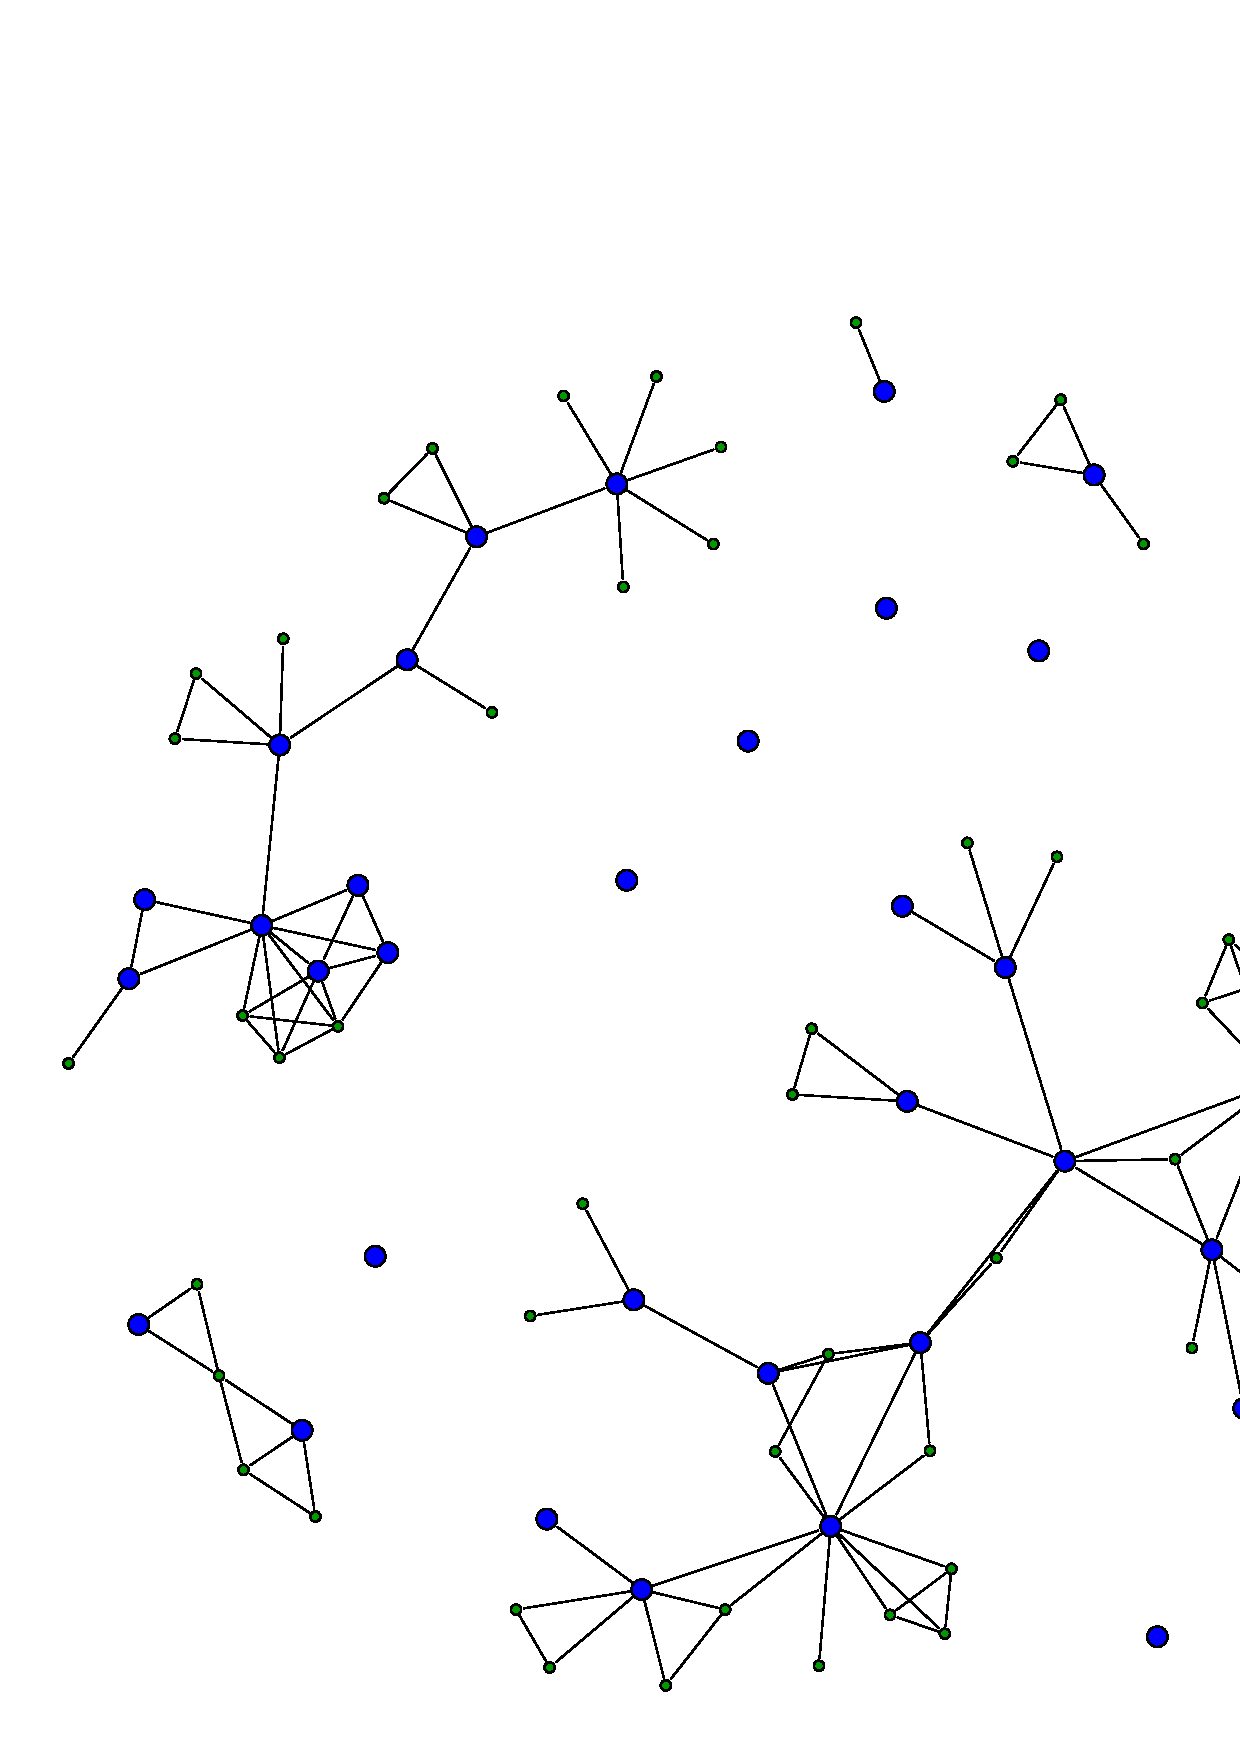
\includegraphics[width=.40\textwidth]{graph} 
  \caption{Descrição da figura mostrada.}
  \label{fig:humanbeta} 
\end{figure}

%% ------------------------------------------------------------------------- %%
\subsection{Aminoácidos}\index{ácido!amino|(}
\label{sec:amino_acidos}

Veja na Tabela \ref{tab:amino_acidos}...  texto texto texto texto texto texto
texto texto texto texto texto texto texto texto texto texto texto texto texto
texto texto texto texto texto texto texto texto texto texto texto texto texto
texto texto texto texto texto texto texto texto texto texto texto texto texto
texto texto texto texto texto texto texto texto texto texto texto.

\begin{table}[!t]
\begin{center}
    \begin{tabular}{c|c|l}
	 \hline
	 Código & Abreviatura & Nome completo \\ \hline
     \texttt{A} & Ala & Alanina \\
     \texttt{C} & Cys & Cisteína \\
     ...        & ... & ... \\
     \texttt{W} & Trp & Tiptofano \\
     \texttt{Y} & Tyr & Tirosina \\ \hline
    \end{tabular}
  \caption{Códigos, abreviaturas e nomes dos aminoácidos.}
  \label{tab:amino_acidos}
\end{center}
\end{table}
\index{ácido!amino|)}

Texto texto texto texto texto texto texto texto texto texto texto texto texto
texto texto texto texto texto texto texto texto texto texto texto texto texto
texto texto texto texto texto texto texto texto texto texto texto texto texto
texto texto texto texto texto texto texto texto texto texto texto texto texto
texto texto texto texto texto texto texto.


%% ------------------------------------------------------------------------- %%
\section{Exemplo de Código-Fonte em Java}
\label{sec:exemplo_codigo_fonte}
Texto texto texto texto texto texto texto texto texto texto texto texto texto
texto texto texto texto texto texto texto texto texto texto texto texto texto
texto texto texto texto texto texto texto texto texto texto texto texto texto
texto texto texto texto texto texto texto.

% Foi utilizado o pacote listing para formatar código fonte
% http://ctan.org/tex-archive/macros/latex/contrib/listings/listings.pdf
% Veja no preambulo do arquivo tese-exemplo.tex os parâmetros de configuração.

\begin{lstlisting}[frame=trbl]
    for(i = 0; i < 20; i++)
    {
        // Comentário 
        System.out.println("Mensagem...");
    }
\end{lstlisting}


%% ------------------------------------------------------------------------- %%
\section{Algumas Referências}
\label{sec:algumas_referencias}

É muito recomendável a utilização de arquivos \emph{bibtex} para o gerenciamento
de referências a trabalhos. Nesse sentido existem três plataformas gratuitas
que permitem a busca de referências acadêmicas em formato bib: 
\begin{itemize}
	\item \emph{CiteULike} (patrocinados por Springer): \url{www.citeulike.org}
	\item Coleção de bibliografia em Ciência da Computação: \url{liinwww.ira.uka.de/bibliography}
	\item Google acadêmico (habilitar bibtex nas preferências): \url{scholar.google.com.br}
\end{itemize}
Lamentavelmente, ainda não existe um mecanismo de verificação ou validação das
informações nessas plataformas. Portanto, é fortemente sugerido validar todas
as informações de tal forma que as entradas bib estejam corretas.  Também, tome
muito cuidado na padronização das referências bibliográficas: ou considere TODOS
os nomes dos autores por extenso, ou TODOS os nomes dos autores abreviados.
Evite misturas inapropriadas.

Exemplos de referências com a tag:
\begin{itemize}
\item @Book: \citep{JW82}.
{\scriptsize\begin{verbatim}
@Book{JW82,
 author   = {Richard A. Johnson and Dean W. Wichern},
 title    = {Applied Multivariate Statistical Analysis},
 publisher= {Prentice-Hall},
 year     = {1983}
}
\end{verbatim}}

\item @Article: \citep{MenaChalco08}.
{\scriptsize\begin{verbatim}
@Article{MenaChalco08,
 author   = {Jesús P. Mena-Chalco and Helaine Carrer and Yossi Zana and 
            Roberto M. Cesar-Jr.},
 title    = {Identification of protein coding regions using the modified 
            {G}abor-wavelet transform},
 journal  = {IEEE/ACM Transactions on Computational Biology and Bioinformatics},
 volume   = {5},
 pages    = {198-207},
 year     = {2008},
}
\end{verbatim}}

\item @InProceedings: \citep{alves03:simi}.
{\scriptsize\begin{verbatim}
@InProceedings{alves03:simi,
 author   = {Carlos E. R. Alves and Edson N. Cáceres and Frank Dehne and 
            Siang W. Song},
 title    = {A Parallel Wavefront Algorithm for Efficient Biological 
            Sequence Comparison},
 booktitle= {ICCSA '03: The 2003 International Conference on Computational Science
            and its Applications},
 year     = {2003},
 pages    = {249-258},
 month    = May,
 publisher= {Springer-Verlag}
}
\end{verbatim}}

\item @InCollection: \citep{bobaoglu93:concepts}.
{\scriptsize\begin{verbatim}
@InCollection{bobaoglu93:concepts,
 author   = {Ozalp Babaoglu and Keith Marzullo},
 title    = {Consistent Global States of Distributed Systems: Fundamental Concepts
            and Mechanisms},
 editor   = {Sape Mullender},
 booktitle= {Distributed Systems},
 edition  = {segunda},
 year     = {1993},
 pages    = {55-96}
}
\end{verbatim}}

\item @Conference: \citep{bronevetsky02}.
{\scriptsize\begin{verbatim}
@Conference{bronevetsky02,
 author   = {Greg Bronevetsky and Daniel Marques and Keshav Pingali and 
            Paul Stodghill},
 title    = {Automated application-level checkpointing of {MPI} programs},
 booktitle= {PPoPP '03: Proceedings of the 9th ACM SIGPLAN Symposium on Principles
            and Practice of Parallel Programming},
 year     = {2003},
 pages    = {84-89}
}
\end{verbatim}}

\item @PhdThesis: \citep{garcia01:PhD}.
{\scriptsize\begin{verbatim}
@PhdThesis{garcia01:PhD,
 author   = {Islene C. Garcia},
 title    = {Visões Progressivas de Computações Distribuídas},
 school   = {Instituto de Computação, Universidade de Campinas, Brasil},
 year     = {2001},
 month    = {Dezembro}
}
\end{verbatim}}

\item @MastersThesis: \citep{schmidt03:MSc}.
{\scriptsize\begin{verbatim}
@MastersThesis{schmidt03:MSc,
 author   = {Rodrigo M. Schmidt},
 title    = {Coleta de Lixo para Protocolos de \emph{Checkpointing}},
 school   = {Instituto de Computação, Universidade de Campinas, Brasil},
 year     = {2003},
 month    = Oct
}
\end{verbatim}}

\item @Techreport: \citep{alvisi99:analysisCIC}.
{\scriptsize\begin{verbatim}
@Techreport{alvisi99:analysisCIC,
 author   = {Lorenzo Alvisi and Elmootazbellah Elnozahy and Sriram S. Rao and
            Syed A. Husain and Asanka Del Mel},
 title    = {An Analysis of Comunication-Induced Checkpointing},
 institution= {Department of Computer Science, University of Texas at Austin},
 year     = {1999},
 number   = {TR-99-01},
 address  = {Austin, {USA}}
}
\end{verbatim}}

\item @Manual: \citep{CORBA:spec}.
{\scriptsize\begin{verbatim}
@Manual{CORBA:spec,
 title    = {{CORBA v3.0 Specification}},
 author   = {{Object Management Group}},
 month    = Jul,
 year     = {2002},
 note     = {{OMG Document 02-06-33}}
}
\end{verbatim}}

\item @Misc: \citep{gridftp}.
{\scriptsize\begin{verbatim}
@Misc{gridftp,
 author   = {William Allcock},
 title    = {{GridFTP} protocol specification. {Global Grid Forum}
            Recommendation ({GFD}.20)},
 year     = {2003}
}
\end{verbatim}}

\item @Misc: para referência a artigo online \citep{fowler04:designDead}.
{\scriptsize\begin{verbatim}
@Misc{fowler04:designDead,
 author   = {Martin Fowler},
 title    = {Is Design Dead?},
 year     = {2004},
 month    = May,
 note     = {Último acesso em 30/1/2010},
 howpublished= {\url{http://martinfowler.com/articles/designDead.html}},
}
\end{verbatim}}

\item @Misc: para referência a página web \citep{FSF:GNU-GPL}.
{\scriptsize\begin{verbatim}
@Misc{FSF:GNU-GPL,
 author   = {Free Software Foundation},
 title    = {GNU general public license},
 year     = {2007},
 note     = {Último acesso em 30/1/2010},
 howpublished= {\url{http://www.gnu.org/copyleft/gpl.html}},
}
\end{verbatim}}

\end{itemize}

         % associado ao arquivo: 'cap-conceitos.tex'
%% ------------------------------------------------------------------------- %%
\chapter{Região de Estudo}
\label{cap:regiao_de_estudo}


Esse capítulo apresenta a região de estudo sob o ponto de vista tectônico e sismológico.

%% ------------------------------------------------------------------------- %%
\section{Contexto Geológico e Tectônico Sul-Americano}
\index{\gls{tectonic}!América do Sul}
\label{sec:03_america_do_sul}

A placa Sul-Americana, como mostra a figura \ref{fig:sa_plate} \citet{bizzi_2003}, tem ao norte a placa do Caribe e a
placa Norte-Americana.
Ao sul estão a placa de Scotia e a placa Antártica. Todas elas se deslocam 
majoritariamente tangencialmente
à placa Sul-Americana.

\begin{figure}[H]
  \centering
  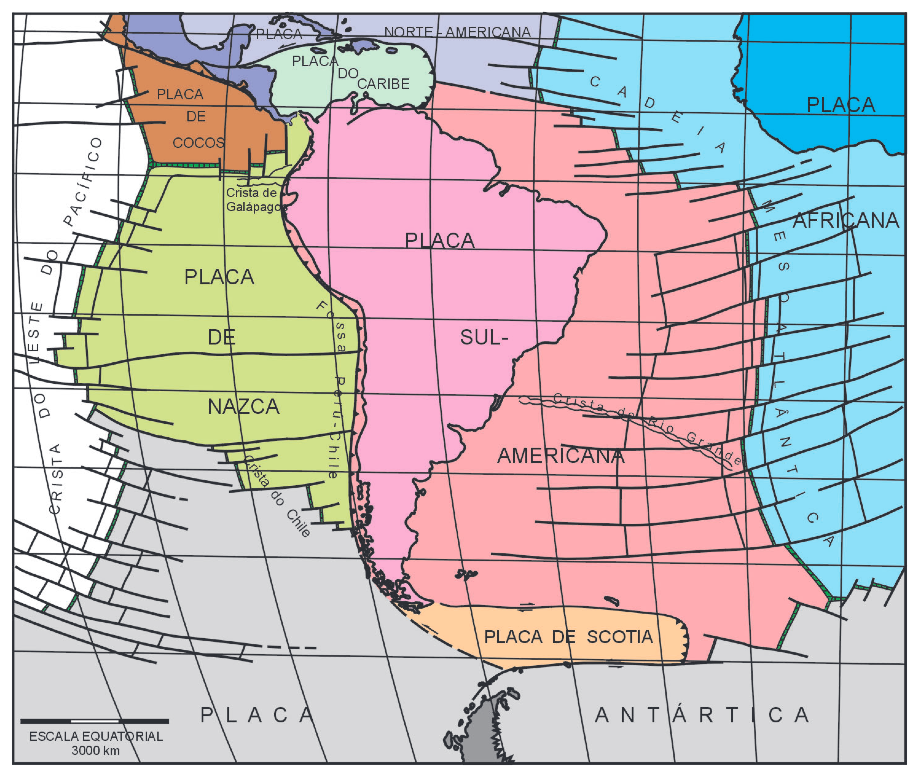
\includegraphics[width=.95\textwidth]{placas_sa} 
  \caption{Placa Sul-Americana em seu contexto global}
  \label{fig:sa_plate} 
\end{figure}


Na divisa com placa Africana à leste está a Dorsal Meso-Atlântica que é resultado
do processo de abertura dos oceanos e separação dos continentes. A abertura dos Atlântico na 
dorsal é responsável por um considerável esforço de compressão horizontal na placa Sul-Americana.

E há também a subducção da placa de Nazca sob a placa Sul-Americana, à oeste,
responsável, entre outros processos, pelo surgimento das Fossas Oceânicas e da
cordilheira dos Andes com suas altitudes e vulcanismo.

Olhando um pouco mais de perto para a parte continental da placa Sul-Americana
(figura \ref{fig:sa_tec}) é interessante destacar três grupos principais de rochas: 
(i) o Embasamento Pré-Cambriano, (ii) as Coberturas Fanerozóicas e (iii) a 
Cadeia Andina.

\begin{figure}[H]
  \centering
  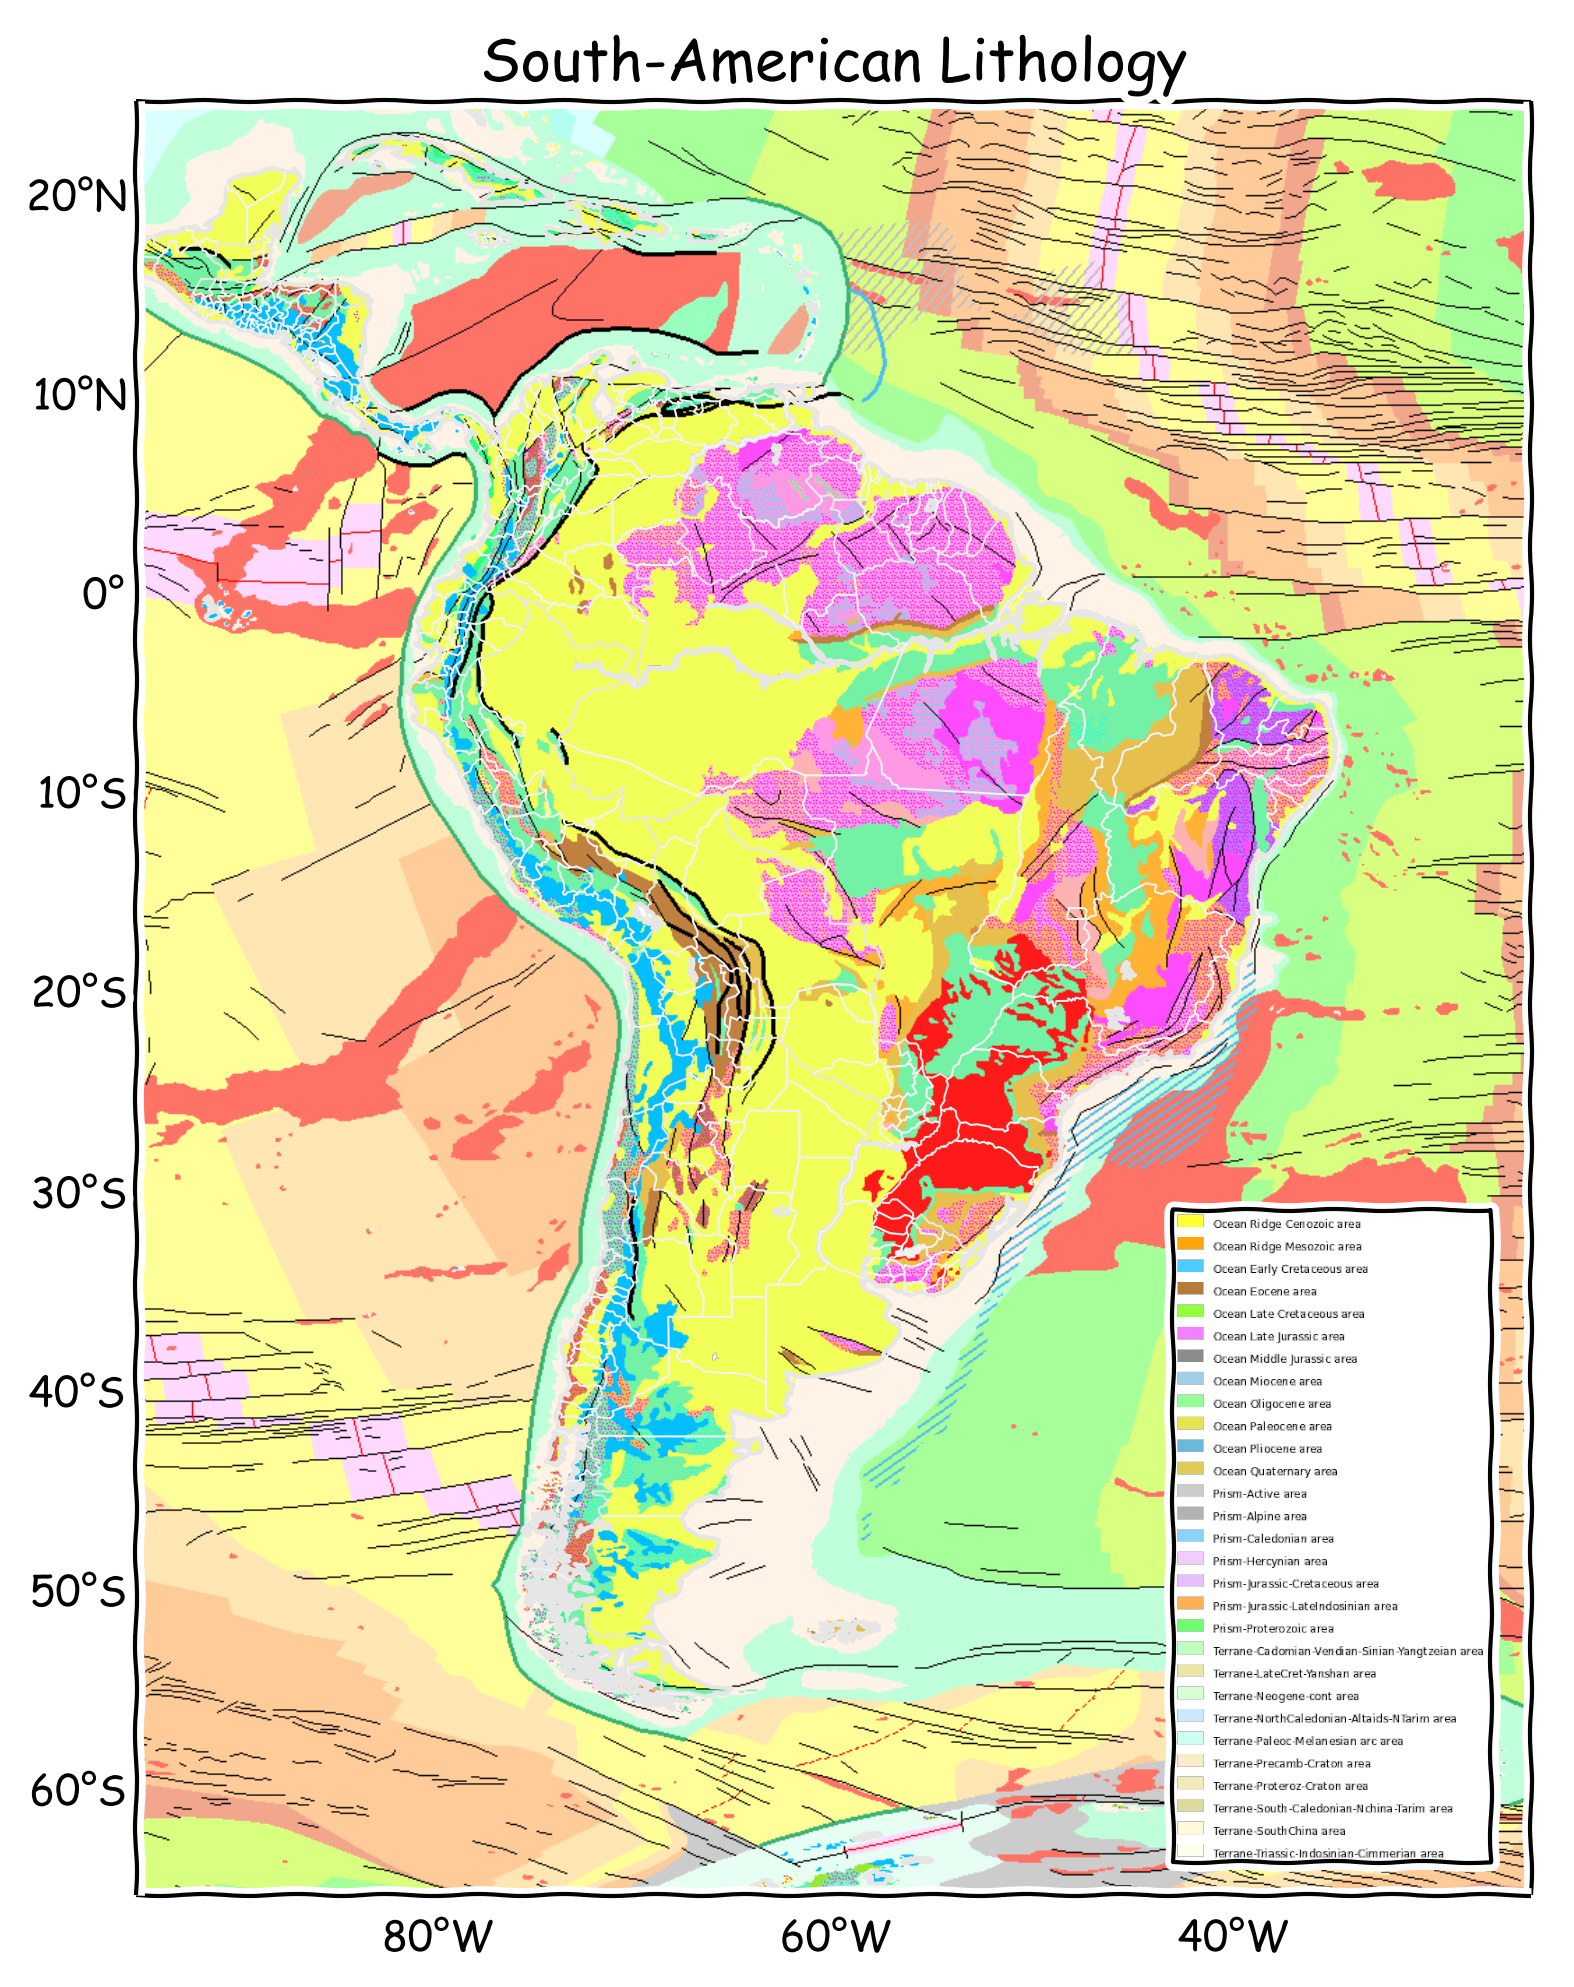
\includegraphics[width=.85\textwidth]{lithology_sa} 
  \caption{Mapa geológico da América do Sul. Fonte \url{http://onegeology.org}}
  \label{fig:sa_tec} 
\end{figure}

As rochas do embasamento pré-cambriano se originaram a mais de 500Ma. Por serem mais antigas
são mais estáveis. A cobertura Fanerozóica é resuldado da sedimentação ocorrida a menos de 250Ma. Formam as bacias
sedimentares. A Cadeia Andina com 30Ma é resultado da subducção e embora exponha rochas pré-cambrianas
em algumas partes é a parte mais ativa e interessante tectonicamente.


\subsubsection{Sismicidade Sul Americana}

A sismicidade Sul-Americana é marcada fortemente pela subducção à oeste e pela 
separação dos oceanos à leste. América Central, Caribe e a parte Antartica ao sul
são placas menores e seus movimentos merecem estudo de maior detalhe.

\begin{figure}[H]
  \centering
  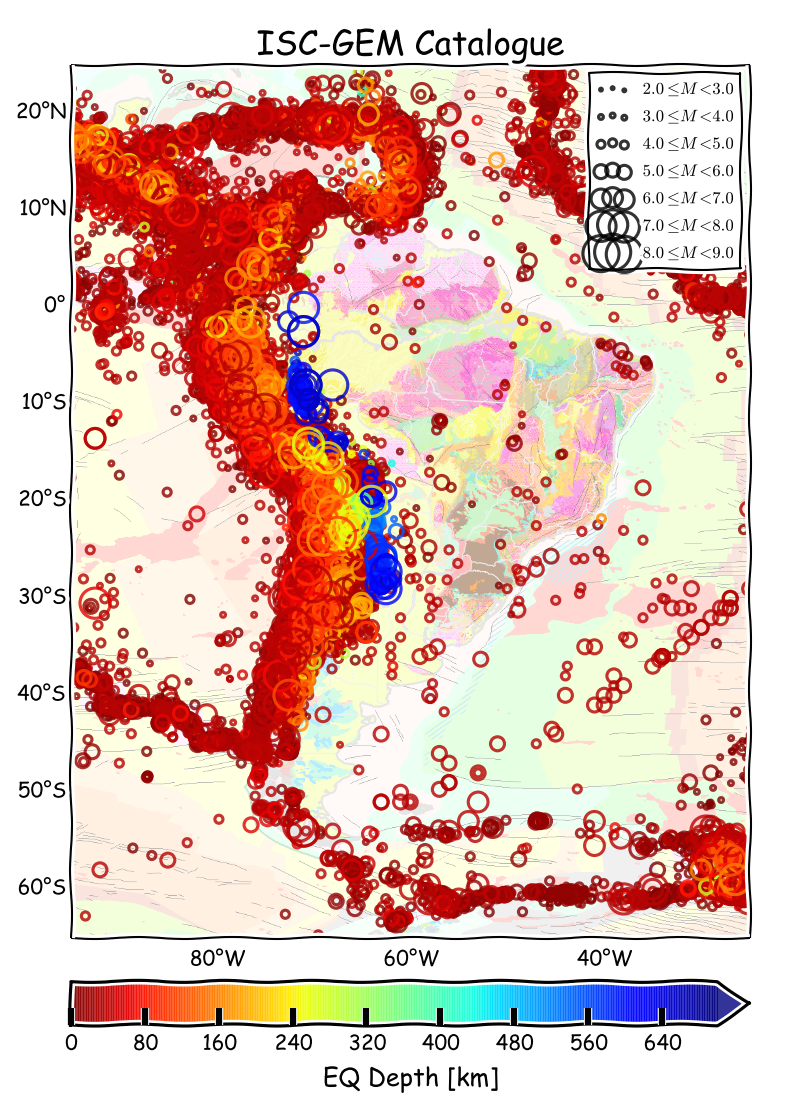
\includegraphics[width=.70\textwidth]{seismicity_sa} 
  \caption{Sismicidade da América do Sul, Catálogo \gls*{iscgem}. 
  		   Geologia: \gls*{cgmw} via OneGeology.
		   Sismos mais profundos foram registrados no interior da placa, inclusive sobre o Acre.
  		   }
  \label{fig:sa_seis} 
\end{figure}

A figura \ref{fig:sa_seis} apresenta a sismicidade da América do Sul pelo catálogo \gls{iscgem}
(seção \ref{sec:data_source}). É possivel notar claramente a subducção, ou seja, do mergulho, da placa de Nazca sob a placa
Sul-Americana. Fica mais claro quando se observa que os sismos com profundidade variando cerca de centenas de
quilômetros e que vão se tornando mais profundos para interior da placa Sul-Americana.

Isso acontece porque parte da quantidade de rocha fria, oceânica e continental, está afundando sob o manto
e lentamente se incorporando à ele. Mas ainda existem atrito, compressões e processos de ruptura nessas
profundidades e que ocorrem majoritariamente na interface entre essas placas pelo acúmulo de tensão e deslocamentos 
mínimos durante milhares de anos e que são liberados instantaneamente na ruptura. 
Esse processo é também o responsável pelo soerguimento da 
cordilheira dos Andes e de boa parte do vulcanismo na região. 

Sismos profundos, de 70 e 700km, geralmente provocam acelerações de baixa intensidade em seus epicentros 
devido à atenuação das ondas.

Também é latente a constatação da diferença de distribuição da sismicidade sul-americana nas bordas de placa e do
resto do continente como um todo. A maior parte do Brasil é praticamente inativa, não desprezível, no histórico
comparado.

%% ------------------------------------------------------------------------- %%
\section{Contexto Geológico e Tectônico Brasileiro}
\index{\gls{tectonic}!Brasil}
\label{sec:geotec_bras}

Tomando-se como referência 500Ma, destacam-se dois grandes grupos de rochas na figura \ref{fig:br_tec}
\citet{bizzi_2003} a seguir.

\begin{figure}[H]
  \centering
  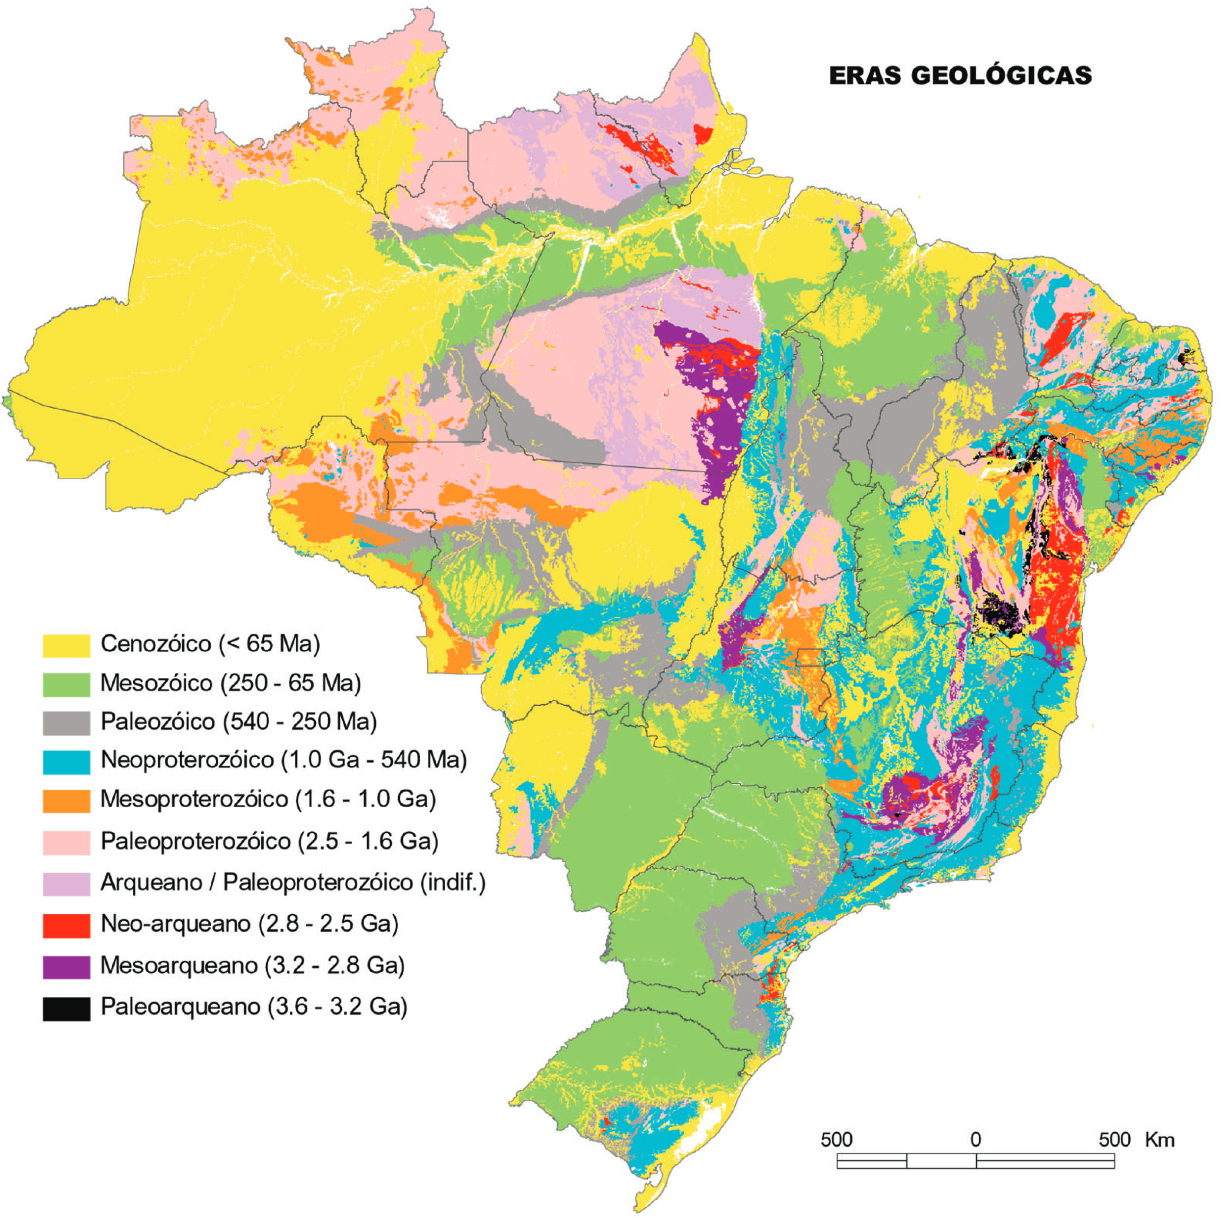
\includegraphics[width=.70\textwidth]{tectonico_brasil} 
  \caption{Mapa Geológico do Brasil em escala 1:1.000.000}.
  \label{fig:br_tec} 
\end{figure}

O embasamento, mais antigo, exposto sob a Amazônia e em porções menores e mais recentes também expostos 
no sudeste e nordeste, cedem espaço à um segundo grupo de rochas mais jovens, fruto da sedimentação e metamorfismos
mais recentes \citep{bizzi_2003}.


%% ------------------------------------------------------------------------- %%
\section{Sismicidade do Brasil}
\index{Sismicidade do Brasil}
\label{sec:sismicidade_brasil}

No Brasil não há terremotos. Não ao menos em quantidade proporcional a 10\% dos sismos sul-americanos.
Mesmo assim, ou por isso mesmo, a ocorrência de um sismo é ainda mais ameaçadora. Onde se espera, 
já se está preparado. Por outro lado onde nunca se espera é sempre uma surpresa.

É fato que o Brasil por estar numa área continental, mais no interior da placa \citep{talwani_2014} e geologia
com uma formação antiga e estável tem um número reduzido, não desprezível, de tremores. 
A figura \ref{fig:br_seis} mostra o detalhe da sismicidade brasileira com a litologia ao fundo.


\begin{figure}[H]
  \centering
  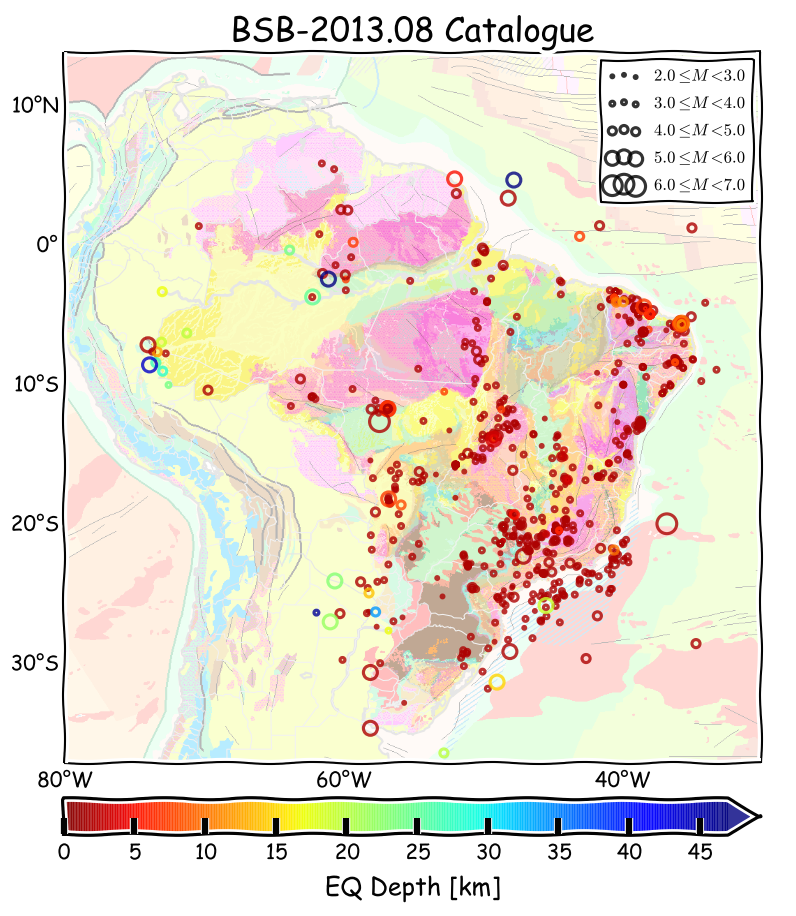
\includegraphics[width=.90\textwidth]{seismicity_br} 
  \caption{Sismicidade do Brasil. Catálogo \gls{bsb2013} (seção \ref{sec:data_source2}).}
  \label{fig:br_seis} 
\end{figure}

É importante notar que já houve registro de sismos com magnitudes pouco acima de 6,
e que sismos de magnitude acima de 4, rasos, em área urbana e em um continente estável,
com baixa atenuação das amplitudes das ondas sísmicas, podem ser danosos.


%% ------------------------------------------------------------------------- %%
\subsection{Sul, Sudeste e Litoral Leste}
\index{Sismicidade do Brasil!sul, sudeste e litoral leste}
\label{sec:z_se}

A sismicidade do sudeste e seu litoral possui características diferentes.
Enquanto no litoral, a principal sismiciade ocorre na área do talude continental
(porção dos fundos marinhos com declive muito pronunciado que fica entre a plataforma continental e
a margem continental e onde começam as planícies abissais), com destaque nessa sismicidade para um dos maiores sismos
que se tem registro no Brasil (figura \ref{fig:z_se}).

\begin{figure}[H]
  \centering
  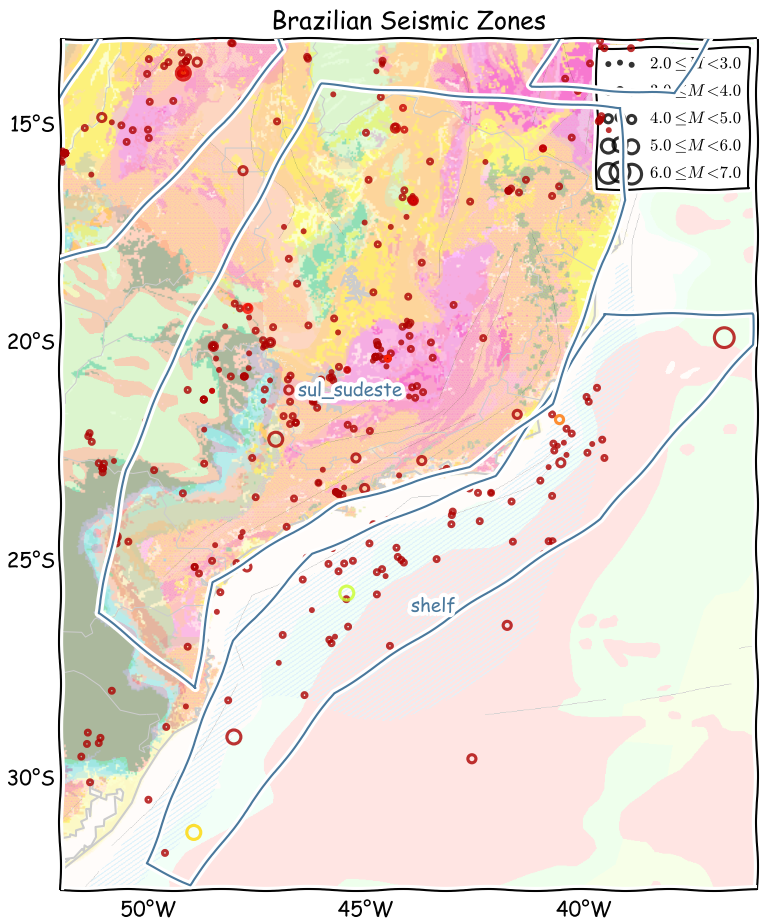
\includegraphics[width=0.6\textwidth]{z_se} 
  \caption{Zona sísmica do SE. \citet{dourado_2014}}
  \label{fig:z_se} 
\end{figure}

O continente é marcado por uma sismicidade difusa na área do cráton que se extende pelo norte de Minas
Gerais até quase o sul da Bahia e outra parte a nordeste da bacia do Paraná. 
Há também uma pequena sismicidade acompanhando a costa. Para maiores referencias, veja 
\citet{assumpcao_2004}.

É nessa região o único registro no Brasil de vítimas fatais decorrentes de tremores de terra, em Itacarambi, MG.

%% ------------------------------------------------------------------------- %%
\subsection{Centro-Norte}
\index{Sismicidade do Brasil!centro-norte}
\label{sec:z_cn}

É uma área com sismicidade peculiar. Na figura \ref{fig:z_cn} De norte a sul acompanha grosseiramente o
contato entre o cráton e parte da bacia do Parnaíba. Também no que seria a 
área central próxima à Chapada dos Veadeiros, em uma outra formação cratônica.

\begin{figure}[H]
  \centering
  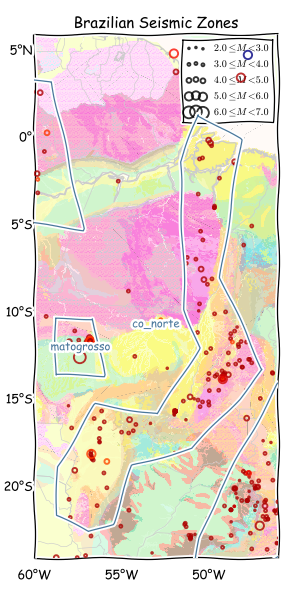
\includegraphics[width=0.45\textwidth]{z_co} 
  \caption{Zona sísmica do Centro-Norte. \citet{dourado_2014}}
  \label{fig:z_cn} 
\end{figure}

A última porção, ao sul, a sismicidade ocorre na área sedimentar da bacia do Pantanal.

%% ------------------------------------------------------------------------- %%
\subsection{Mato-Grosso}
\index{Sismicidade do Brasil!centro-norte}
\label{sec:z_mt}

A sismicidade do Mato-Grosso, mais precisamente de Porto-de-Gaúchos (\ref{fig:z_mt}), é emblemática para o Brasil.
Poderia ser considerada com características similares a Nova Madri, EUA.

\begin{figure}[H]
  \centering
  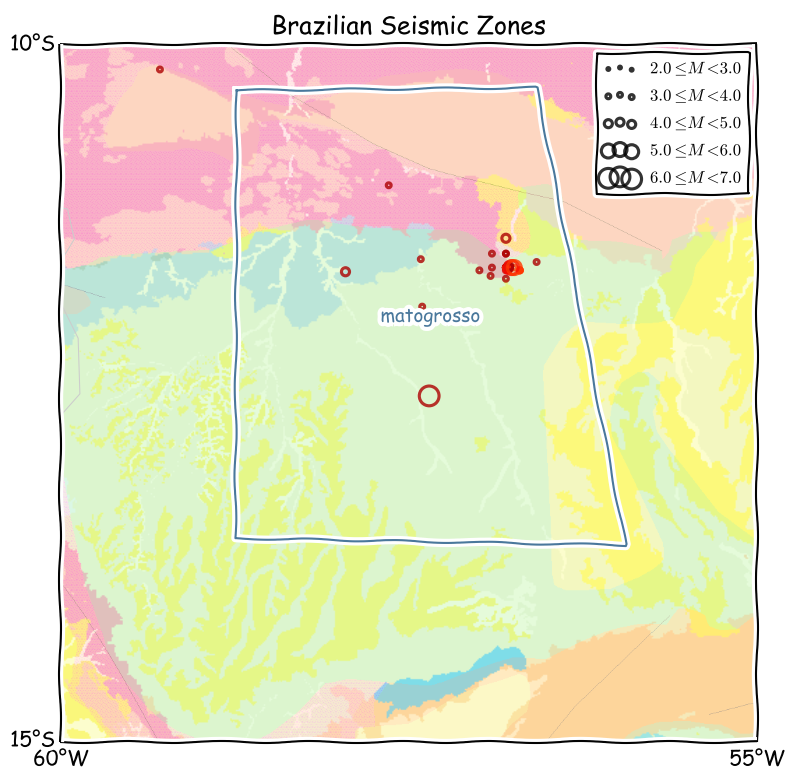
\includegraphics[width=0.45\textwidth]{z_mt} 
  \caption{Zona sísmica do Centro-Norte. \citet{dourado_2014}}
  \label{fig:z_mt} 
\end{figure}

A região sofreu um dos maiores sismos já registrados no Brasil, com magnitude pouco acima de 6.
Não há registros de falhas geológicas neo-tectônicas e mais complexa de ser explicada \citep{barros_2009}.

%% ------------------------------------------------------------------------- %%
\subsection{Extremo Oeste e Acre}
\index{Sismicidade do Brasil!extremo-oeste}
\label{sec:z_ac}

No extremo oeste do Brasil, na região do Acre, a sismicidade tem uma característica distinta das outras.
É possível reparar, na figura \ref{fig:z_ac}, primeiramente na quantidade de sismos, e em
seguida perceber a influência dos sismos sul americanos, desde os mais profundos aos intermediários
e relativamente rasos de 70km. 


\begin{figure}[H]
  \centering
  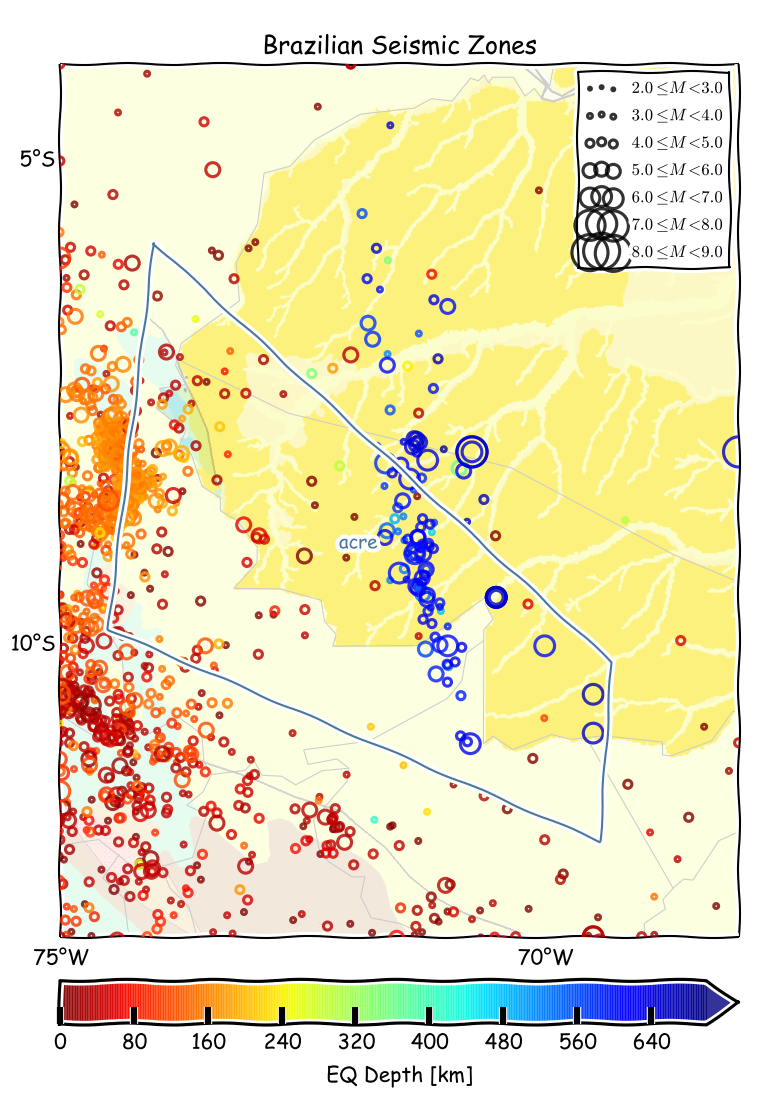
\includegraphics[width=0.5\textwidth]{z_ac} 
  \caption{Zona sísmica do Acre. Dourado}
  \label{fig:z_ac} 
\end{figure}

Note que a escala de profundidade da figura \ref{fig:z_ac} é diferente das demais que seguem a
mesma escala da figura \ref{fig:br_seis}.


%% ------------------------------------------------------------------------- %%
\subsection{Amazonas}
\index{Sismicidade do Brasil!Amazonas}
\label{sec:z_am}

É a região com menor quantidade de conhecimento e informação disponível.
Ainda assim, na figura \ref{fig:z_am} é possível observar a ocorrência de sismos
na direção norte-sul.

\begin{figure}[H]
  \centering
  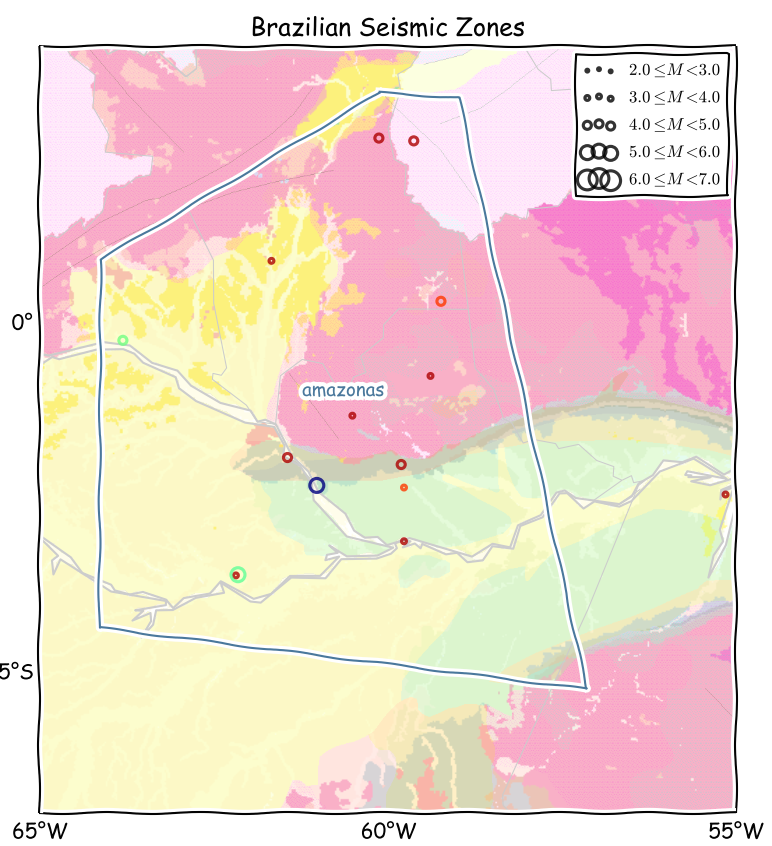
\includegraphics[width=0.5\textwidth]{z_am} 
  \caption{Zona sísmica de Manaus. Dourado}
  \label{fig:z_am} 
\end{figure}

O registro de um sismo de magnitude 5 determinada por dados macrossísmicos,
é o indício mais marcante na região.


%% ------------------------------------------------------------------------- %%
\subsection{Nordeste}
\index{Sismicidade do Brasil!nordeste}
\label{sec:z_ne}

A regisão nordeste brasileira é sismicamente a mais ativa (figura \ref{fig:z_ne}). 

\begin{figure}[H]
  \centering
  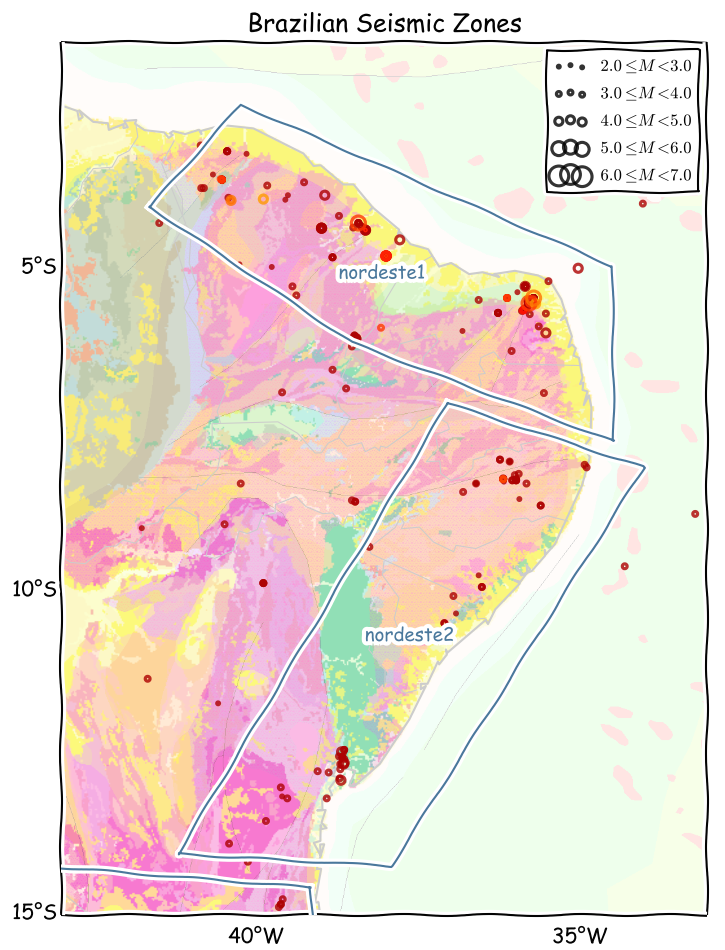
\includegraphics[width=0.6\textwidth]{z_ne} 
  \caption{Zona sísmica do NE. \citet{dourado_2014}}
  \label{fig:z_ne} 
\end{figure}

Destaca-se a sismicidade na região de João Câmara no Rio Grande do Norte,
com um enxame sísmico em meados da década de 1980 \citep{takeya_1989, bezerra_1998}. 
Além disso são bem conhecidas as atividades sísmicas na região de Sobral-CE,
na região de Pernambuco e um pouco mais ao sul já na Bahia.


        	  % associado ao arquivo: 'cap-conclusoes.tex'
%% ------------------------------------------------------------------------- %%
\chapter{Conceitos}
\label{cap:conceitos}

Texto texto texto texto texto texto texto texto texto texto texto texto texto
texto texto texto texto texto texto texto texto texto texto texto texto texto
texto texto texto texto texto texto texto texto texto texto texto texto texto
texto texto texto texto texto texto texto texto texto texto texto texto texto
texto texto texto texto texto texto.

%% ------------------------------------------------------------------------- %%
\section{Fundamentos}\index{área do trabalho!fundamentos}
\label{sec:fundamentos}

Texto texto texto texto texto texto texto texto texto texto texto texto texto
texto texto texto texto texto texto texto texto texto texto texto texto texto
texto texto texto texto texto texto texto texto texto texto texto texto texto
texto texto texto texto texto texto texto texto texto texto texto texto texto
texto texto texto.

%% ------------------------------------------------------------------------- %%
\subsection{Ácidos Nucléicos}\index{ácido!nucléico}\index{nucleotídeos}
\label{sec:acidos_nucleicos}

Na Figura~\ref{fig:humanbeta} texto texto texto texto texto texto texto texto
texto texto texto texto texto texto texto texto texto texto texto texto texto
texto texto texto texto texto texto texto texto texto texto texto texto texto
texto texto texto texto texto texto texto texto texto texto texto texto texto
texto texto texto.

\begin{figure}[!h]
  \centering
  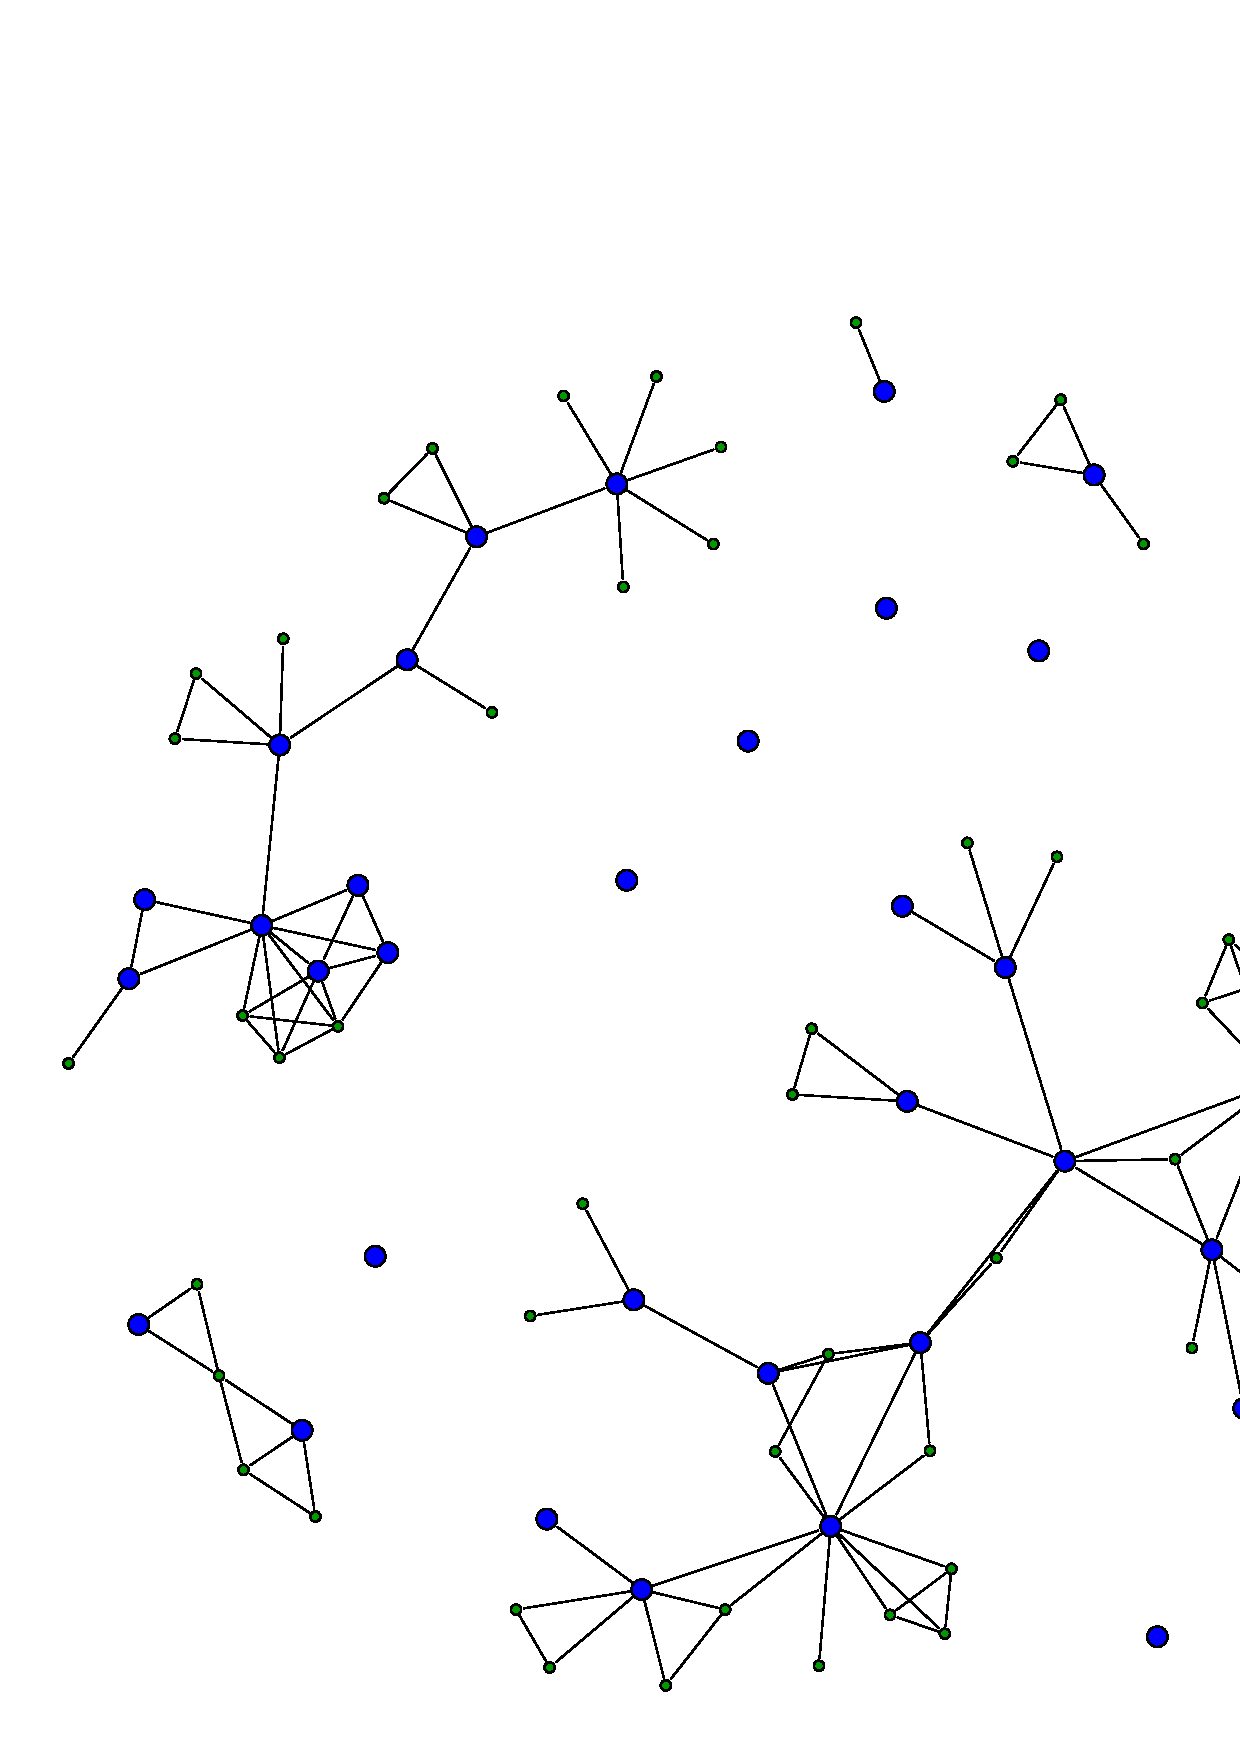
\includegraphics[width=.40\textwidth]{graph} 
  \caption{Descrição da figura mostrada.}
  \label{fig:humanbeta} 
\end{figure}

%% ------------------------------------------------------------------------- %%
\subsection{Aminoácidos}\index{ácido!amino|(}
\label{sec:amino_acidos}

Veja na Tabela \ref{tab:amino_acidos}...  texto texto texto texto texto texto
texto texto texto texto texto texto texto texto texto texto texto texto texto
texto texto texto texto texto texto texto texto texto texto texto texto texto
texto texto texto texto texto texto texto texto texto texto texto texto texto
texto texto texto texto texto texto texto texto texto texto texto.

\begin{table}[!t]
\begin{center}
    \begin{tabular}{c|c|l}
	 \hline
	 Código & Abreviatura & Nome completo \\ \hline
     \texttt{A} & Ala & Alanina \\
     \texttt{C} & Cys & Cisteína \\
     ...        & ... & ... \\
     \texttt{W} & Trp & Tiptofano \\
     \texttt{Y} & Tyr & Tirosina \\ \hline
    \end{tabular}
  \caption{Códigos, abreviaturas e nomes dos aminoácidos.}
  \label{tab:amino_acidos}
\end{center}
\end{table}
\index{ácido!amino|)}

Texto texto texto texto texto texto texto texto texto texto texto texto texto
texto texto texto texto texto texto texto texto texto texto texto texto texto
texto texto texto texto texto texto texto texto texto texto texto texto texto
texto texto texto texto texto texto texto texto texto texto texto texto texto
texto texto texto texto texto texto texto.


%% ------------------------------------------------------------------------- %%
\section{Exemplo de Código-Fonte em Java}
\label{sec:exemplo_codigo_fonte}
Texto texto texto texto texto texto texto texto texto texto texto texto texto
texto texto texto texto texto texto texto texto texto texto texto texto texto
texto texto texto texto texto texto texto texto texto texto texto texto texto
texto texto texto texto texto texto texto.

% Foi utilizado o pacote listing para formatar código fonte
% http://ctan.org/tex-archive/macros/latex/contrib/listings/listings.pdf
% Veja no preambulo do arquivo tese-exemplo.tex os parâmetros de configuração.

\begin{lstlisting}[frame=trbl]
    for(i = 0; i < 20; i++)
    {
        // Comentário 
        System.out.println("Mensagem...");
    }
\end{lstlisting}


%% ------------------------------------------------------------------------- %%
\section{Algumas Referências}
\label{sec:algumas_referencias}

É muito recomendável a utilização de arquivos \emph{bibtex} para o gerenciamento
de referências a trabalhos. Nesse sentido existem três plataformas gratuitas
que permitem a busca de referências acadêmicas em formato bib: 
\begin{itemize}
	\item \emph{CiteULike} (patrocinados por Springer): \url{www.citeulike.org}
	\item Coleção de bibliografia em Ciência da Computação: \url{liinwww.ira.uka.de/bibliography}
	\item Google acadêmico (habilitar bibtex nas preferências): \url{scholar.google.com.br}
\end{itemize}
Lamentavelmente, ainda não existe um mecanismo de verificação ou validação das
informações nessas plataformas. Portanto, é fortemente sugerido validar todas
as informações de tal forma que as entradas bib estejam corretas.  Também, tome
muito cuidado na padronização das referências bibliográficas: ou considere TODOS
os nomes dos autores por extenso, ou TODOS os nomes dos autores abreviados.
Evite misturas inapropriadas.

Exemplos de referências com a tag:
\begin{itemize}


\item @Article: \citep{MenaChalco08}.
{\scriptsize\begin{verbatim}
@Article{MenaChalco08,
 author   = {Jesús P. Mena-Chalco and Helaine Carrer and Yossi Zana and 
            Roberto M. Cesar-Jr.},
 title    = {Identification of protein coding regions using the modified 
            {G}abor-wavelet transform},
 journal  = {IEEE/ACM Transactions on Computational Biology and Bioinformatics},
 volume   = {5},
 pages    = {198-207},
 year     = {2008},
}
\end{verbatim}}


\end{itemize}

       % associado ao arquivo: 'cap-introducao.tex'
%% ------------------------------------------------------------------------- %%
\chapter{Conceitos}
\label{cap:conceitos}

Texto texto texto texto texto texto texto texto texto texto texto texto texto
texto texto texto texto texto texto texto texto texto texto texto texto texto
texto texto texto texto texto texto texto texto texto texto texto texto texto
texto texto texto texto texto texto texto texto texto texto texto texto texto
texto texto texto texto texto texto.

%% ------------------------------------------------------------------------- %%
\section{Fundamentos}\index{área do trabalho!fundamentos}
\label{sec:fundamentos}

Texto texto texto texto texto texto texto texto texto texto texto texto texto
texto texto texto texto texto texto texto texto texto texto texto texto texto
texto texto texto texto texto texto texto texto texto texto texto texto texto
texto texto texto texto texto texto texto texto texto texto texto texto texto
texto texto texto.

%% ------------------------------------------------------------------------- %%
\subsection{Ácidos Nucléicos}\index{ácido!nucléico}\index{nucleotídeos}
\label{sec:acidos_nucleicos}

Na Figura~\ref{fig:humanbeta} texto texto texto texto texto texto texto texto
texto texto texto texto texto texto texto texto texto texto texto texto texto
texto texto texto texto texto texto texto texto texto texto texto texto texto
texto texto texto texto texto texto texto texto texto texto texto texto texto
texto texto texto.

\begin{figure}[!h]
  \centering
  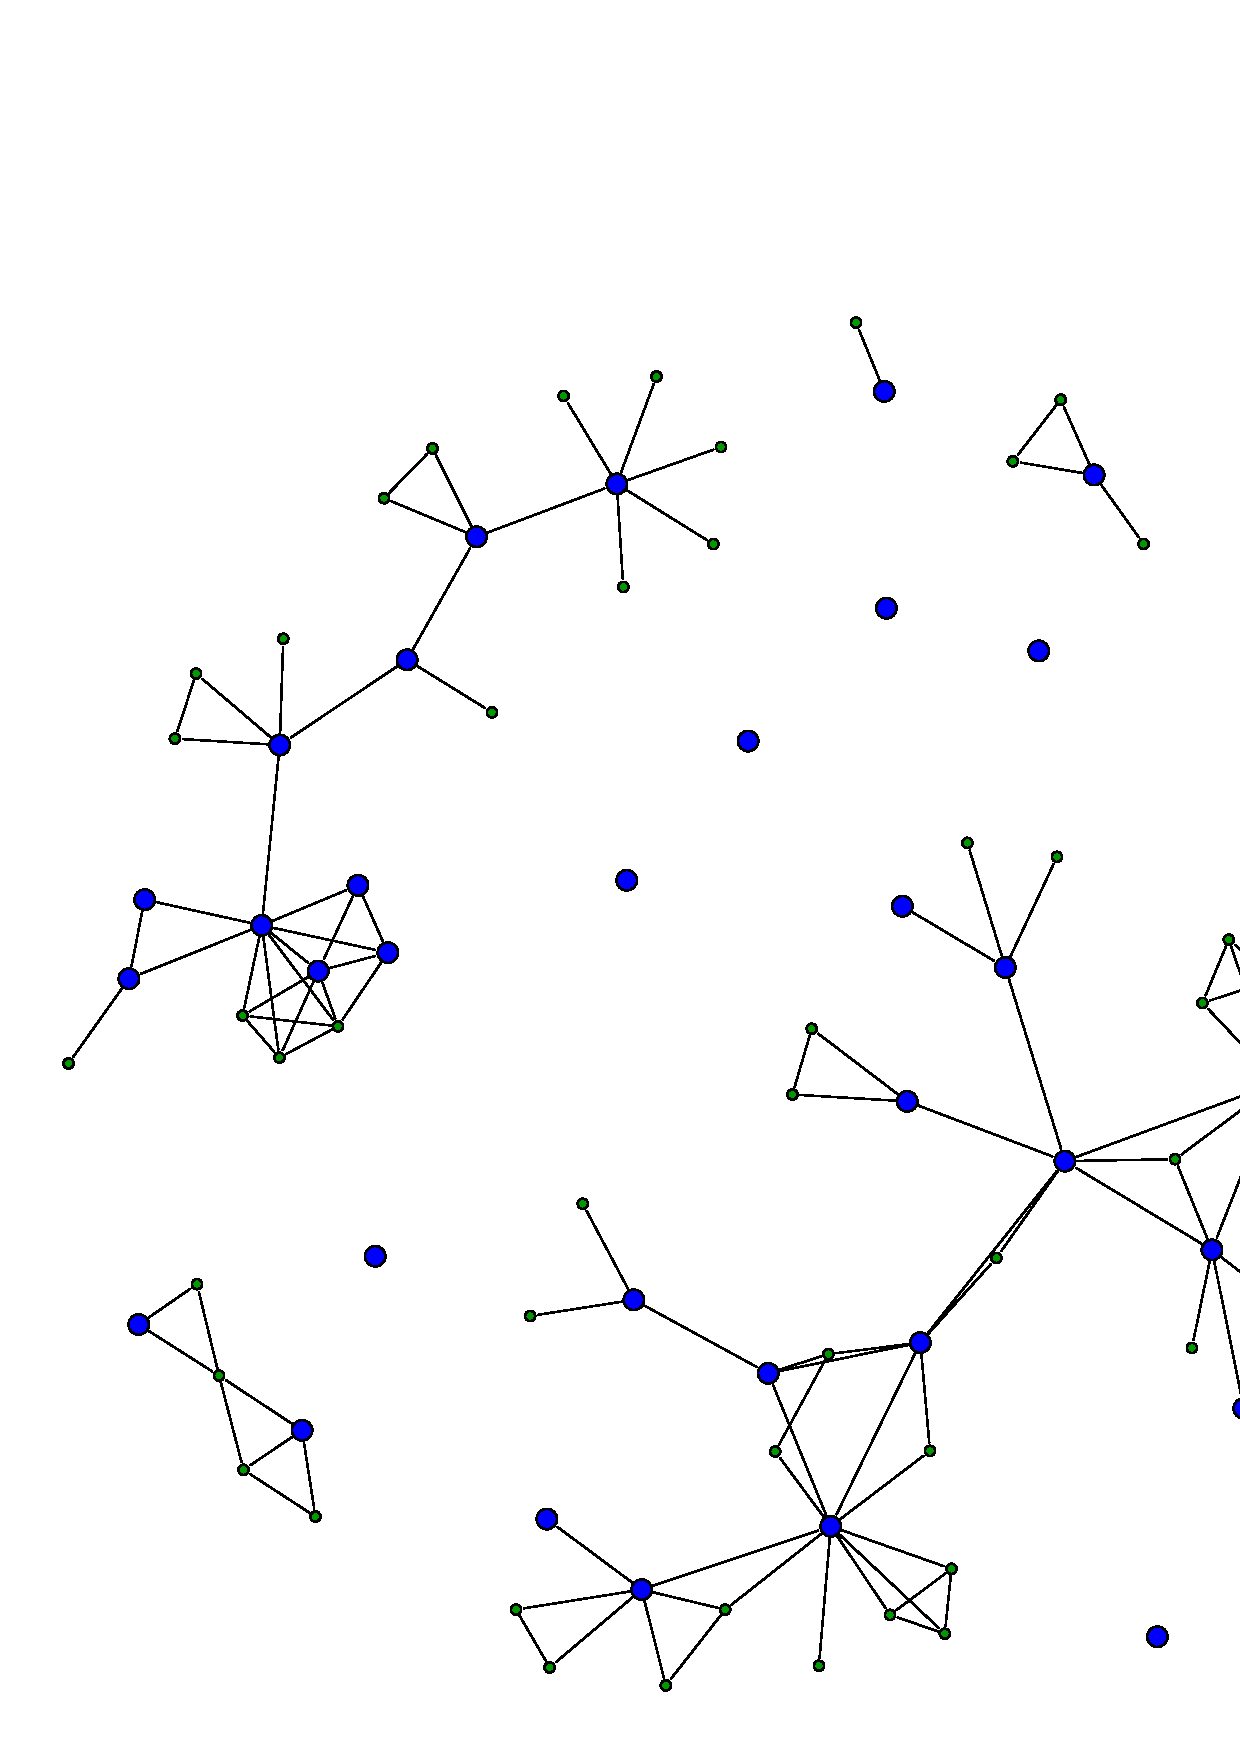
\includegraphics[width=.40\textwidth]{graph} 
  \caption{Descrição da figura mostrada.}
  \label{fig:humanbeta} 
\end{figure}

%% ------------------------------------------------------------------------- %%
\subsection{Aminoácidos}\index{ácido!amino|(}
\label{sec:amino_acidos}

Veja na Tabela \ref{tab:amino_acidos}...  texto texto texto texto texto texto
texto texto texto texto texto texto texto texto texto texto texto texto texto
texto texto texto texto texto texto texto texto texto texto texto texto texto
texto texto texto texto texto texto texto texto texto texto texto texto texto
texto texto texto texto texto texto texto texto texto texto texto.

\begin{table}[!t]
\begin{center}
    \begin{tabular}{c|c|l}
	 \hline
	 Código & Abreviatura & Nome completo \\ \hline
     \texttt{A} & Ala & Alanina \\
     \texttt{C} & Cys & Cisteína \\
     ...        & ... & ... \\
     \texttt{W} & Trp & Tiptofano \\
     \texttt{Y} & Tyr & Tirosina \\ \hline
    \end{tabular}
  \caption{Códigos, abreviaturas e nomes dos aminoácidos.}
  \label{tab:amino_acidos}
\end{center}
\end{table}
\index{ácido!amino|)}

Texto texto texto texto texto texto texto texto texto texto texto texto texto
texto texto texto texto texto texto texto texto texto texto texto texto texto
texto texto texto texto texto texto texto texto texto texto texto texto texto
texto texto texto texto texto texto texto texto texto texto texto texto texto
texto texto texto texto texto texto texto.


%% ------------------------------------------------------------------------- %%
\section{Exemplo de Código-Fonte em Java}
\label{sec:exemplo_codigo_fonte}
Texto texto texto texto texto texto texto texto texto texto texto texto texto
texto texto texto texto texto texto texto texto texto texto texto texto texto
texto texto texto texto texto texto texto texto texto texto texto texto texto
texto texto texto texto texto texto texto.

% Foi utilizado o pacote listing para formatar código fonte
% http://ctan.org/tex-archive/macros/latex/contrib/listings/listings.pdf
% Veja no preambulo do arquivo tese-exemplo.tex os parâmetros de configuração.

\begin{lstlisting}[frame=trbl]
    for(i = 0; i < 20; i++)
    {
        // Comentário 
        System.out.println("Mensagem...");
    }
\end{lstlisting}


%% ------------------------------------------------------------------------- %%
\section{Algumas Referências}
\label{sec:algumas_referencias}

É muito recomendável a utilização de arquivos \emph{bibtex} para o gerenciamento
de referências a trabalhos. Nesse sentido existem três plataformas gratuitas
que permitem a busca de referências acadêmicas em formato bib: 
\begin{itemize}
	\item \emph{CiteULike} (patrocinados por Springer): \url{www.citeulike.org}
	\item Coleção de bibliografia em Ciência da Computação: \url{liinwww.ira.uka.de/bibliography}
	\item Google acadêmico (habilitar bibtex nas preferências): \url{scholar.google.com.br}
\end{itemize}
Lamentavelmente, ainda não existe um mecanismo de verificação ou validação das
informações nessas plataformas. Portanto, é fortemente sugerido validar todas
as informações de tal forma que as entradas bib estejam corretas.  Também, tome
muito cuidado na padronização das referências bibliográficas: ou considere TODOS
os nomes dos autores por extenso, ou TODOS os nomes dos autores abreviados.
Evite misturas inapropriadas.

Exemplos de referências com a tag:
\begin{itemize}


\item @Article: \citep{MenaChalco08}.
{\scriptsize\begin{verbatim}
@Article{MenaChalco08,
 author   = {Jesús P. Mena-Chalco and Helaine Carrer and Yossi Zana and 
            Roberto M. Cesar-Jr.},
 title    = {Identification of protein coding regions using the modified 
            {G}abor-wavelet transform},
 journal  = {IEEE/ACM Transactions on Computational Biology and Bioinformatics},
 volume   = {5},
 pages    = {198-207},
 year     = {2008},
}
\end{verbatim}}


\end{itemize}

     % associado ao arquivo: 'cap-conceitos.tex'
%% ------------------------------------------------------------------------- %%
\chapter{Conceitos}
\label{cap:conceitos}

Texto texto texto texto texto texto texto texto texto texto texto texto texto
texto texto texto texto texto texto texto texto texto texto texto texto texto
texto texto texto texto texto texto texto texto texto texto texto texto texto
texto texto texto texto texto texto texto texto texto texto texto texto texto
texto texto texto texto texto texto.

%% ------------------------------------------------------------------------- %%
\section{Fundamentos}\index{área do trabalho!fundamentos}
\label{sec:fundamentos}

Texto texto texto texto texto texto texto texto texto texto texto texto texto
texto texto texto texto texto texto texto texto texto texto texto texto texto
texto texto texto texto texto texto texto texto texto texto texto texto texto
texto texto texto texto texto texto texto texto texto texto texto texto texto
texto texto texto.

%% ------------------------------------------------------------------------- %%
\subsection{Ácidos Nucléicos}\index{ácido!nucléico}\index{nucleotídeos}
\label{sec:acidos_nucleicos}

Na Figura~\ref{fig:humanbeta} texto texto texto texto texto texto texto texto
texto texto texto texto texto texto texto texto texto texto texto texto texto
texto texto texto texto texto texto texto texto texto texto texto texto texto
texto texto texto texto texto texto texto texto texto texto texto texto texto
texto texto texto.

\begin{figure}[!h]
  \centering
  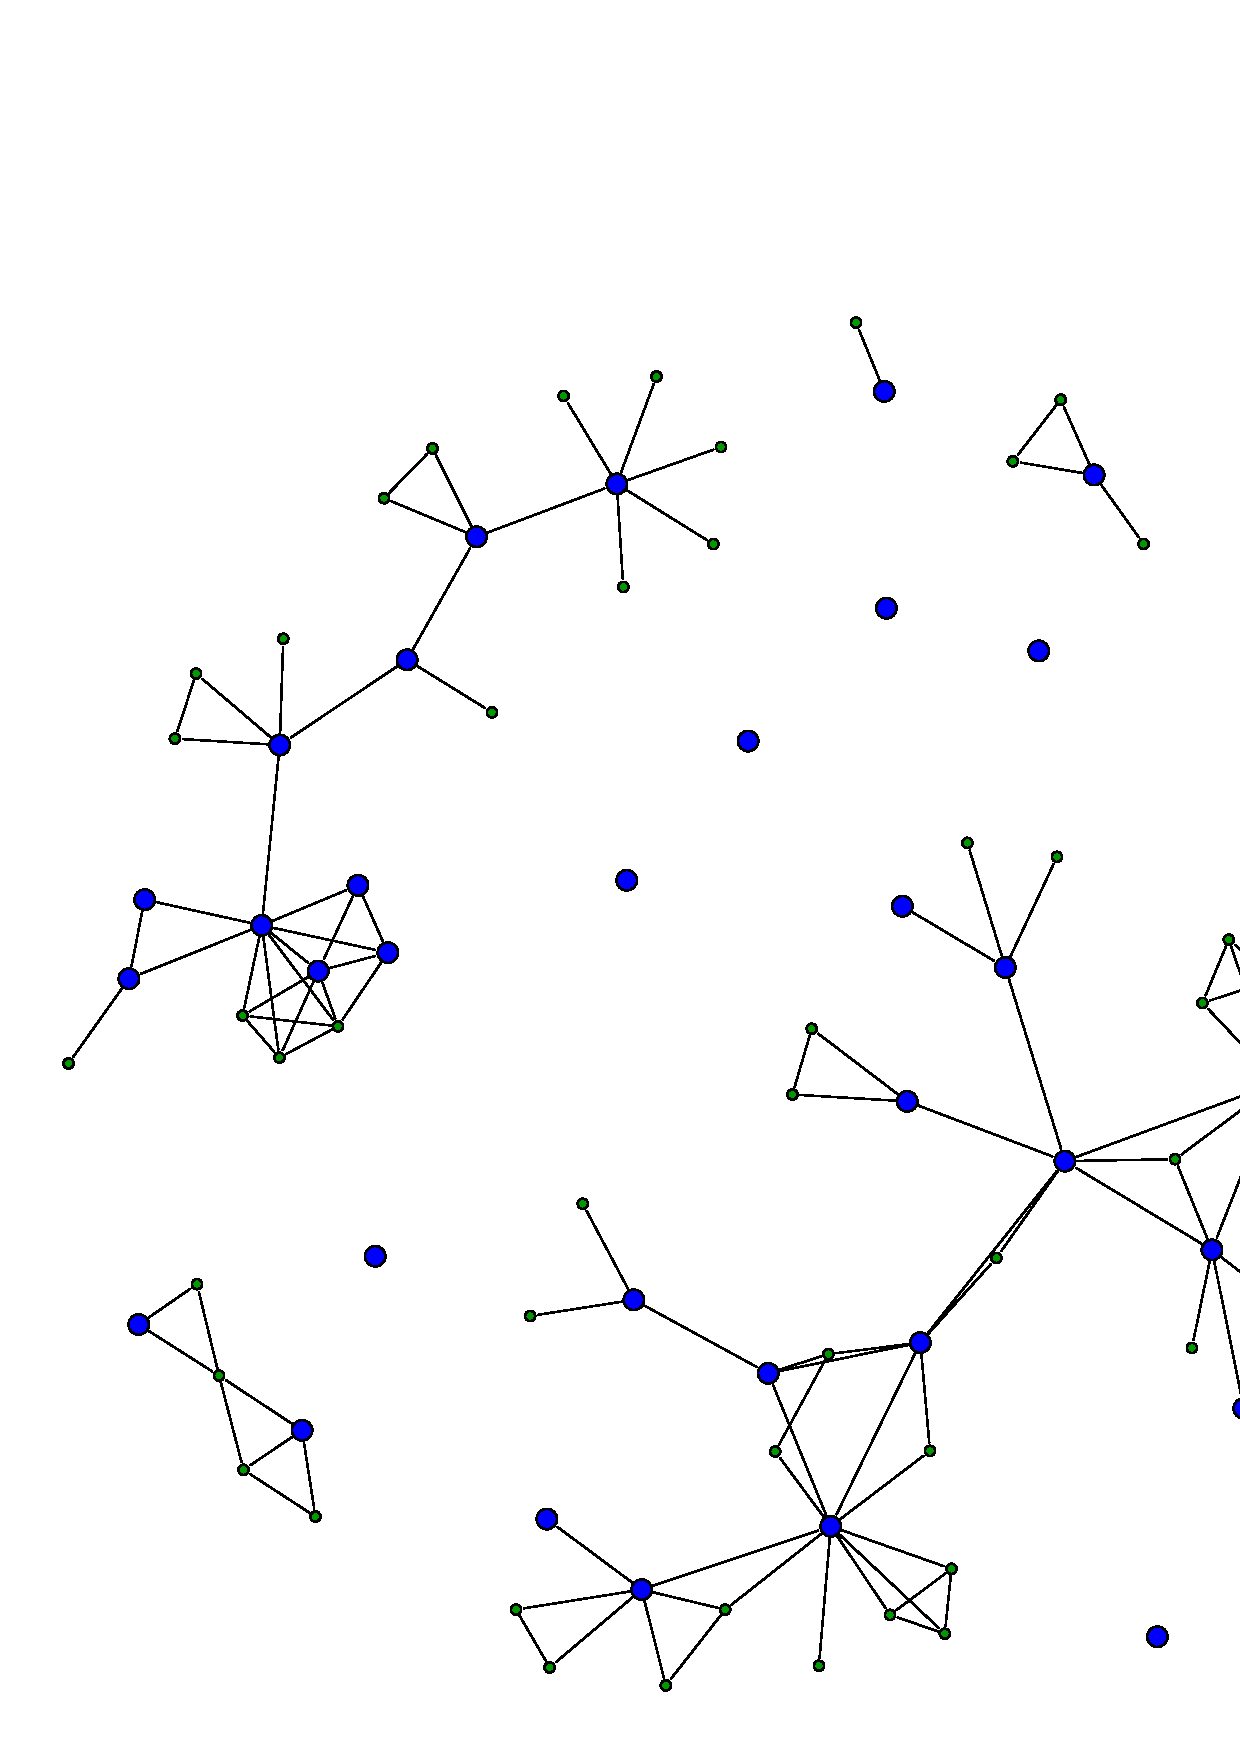
\includegraphics[width=.40\textwidth]{graph} 
  \caption{Descrição da figura mostrada.}
  \label{fig:humanbeta} 
\end{figure}

%% ------------------------------------------------------------------------- %%
\subsection{Aminoácidos}\index{ácido!amino|(}
\label{sec:amino_acidos}

Veja na Tabela \ref{tab:amino_acidos}...  texto texto texto texto texto texto
texto texto texto texto texto texto texto texto texto texto texto texto texto
texto texto texto texto texto texto texto texto texto texto texto texto texto
texto texto texto texto texto texto texto texto texto texto texto texto texto
texto texto texto texto texto texto texto texto texto texto texto.

\begin{table}[!t]
\begin{center}
    \begin{tabular}{c|c|l}
	 \hline
	 Código & Abreviatura & Nome completo \\ \hline
     \texttt{A} & Ala & Alanina \\
     \texttt{C} & Cys & Cisteína \\
     ...        & ... & ... \\
     \texttt{W} & Trp & Tiptofano \\
     \texttt{Y} & Tyr & Tirosina \\ \hline
    \end{tabular}
  \caption{Códigos, abreviaturas e nomes dos aminoácidos.}
  \label{tab:amino_acidos}
\end{center}
\end{table}
\index{ácido!amino|)}

Texto texto texto texto texto texto texto texto texto texto texto texto texto
texto texto texto texto texto texto texto texto texto texto texto texto texto
texto texto texto texto texto texto texto texto texto texto texto texto texto
texto texto texto texto texto texto texto texto texto texto texto texto texto
texto texto texto texto texto texto texto.


%% ------------------------------------------------------------------------- %%
\section{Exemplo de Código-Fonte em Java}
\label{sec:exemplo_codigo_fonte}
Texto texto texto texto texto texto texto texto texto texto texto texto texto
texto texto texto texto texto texto texto texto texto texto texto texto texto
texto texto texto texto texto texto texto texto texto texto texto texto texto
texto texto texto texto texto texto texto.

% Foi utilizado o pacote listing para formatar código fonte
% http://ctan.org/tex-archive/macros/latex/contrib/listings/listings.pdf
% Veja no preambulo do arquivo tese-exemplo.tex os parâmetros de configuração.

\begin{lstlisting}[frame=trbl]
    for(i = 0; i < 20; i++)
    {
        // Comentário 
        System.out.println("Mensagem...");
    }
\end{lstlisting}


%% ------------------------------------------------------------------------- %%
\section{Algumas Referências}
\label{sec:algumas_referencias}

É muito recomendável a utilização de arquivos \emph{bibtex} para o gerenciamento
de referências a trabalhos. Nesse sentido existem três plataformas gratuitas
que permitem a busca de referências acadêmicas em formato bib: 
\begin{itemize}
	\item \emph{CiteULike} (patrocinados por Springer): \url{www.citeulike.org}
	\item Coleção de bibliografia em Ciência da Computação: \url{liinwww.ira.uka.de/bibliography}
	\item Google acadêmico (habilitar bibtex nas preferências): \url{scholar.google.com.br}
\end{itemize}
Lamentavelmente, ainda não existe um mecanismo de verificação ou validação das
informações nessas plataformas. Portanto, é fortemente sugerido validar todas
as informações de tal forma que as entradas bib estejam corretas.  Também, tome
muito cuidado na padronização das referências bibliográficas: ou considere TODOS
os nomes dos autores por extenso, ou TODOS os nomes dos autores abreviados.
Evite misturas inapropriadas.

Exemplos de referências com a tag:
\begin{itemize}


\item @Article: \citep{MenaChalco08}.
{\scriptsize\begin{verbatim}
@Article{MenaChalco08,
 author   = {Jesús P. Mena-Chalco and Helaine Carrer and Yossi Zana and 
            Roberto M. Cesar-Jr.},
 title    = {Identification of protein coding regions using the modified 
            {G}abor-wavelet transform},
 journal  = {IEEE/ACM Transactions on Computational Biology and Bioinformatics},
 volume   = {5},
 pages    = {198-207},
 year     = {2008},
}
\end{verbatim}}


\end{itemize}

        % associado ao arquivo: 'cap-conclusoes.tex'
%% ------------------------------------------------------------------------- %%
\chapter{Discussão}
\label{cap:conclusoes}

Apesar de possuirem implementações distintas de um mesmo fundamento matemático e estatítstico
que é a estimativa de densidade por funções de núcleo, os métodos, no geral, conseguiram
estimar das características da sismicidade a partir da sismicidade histórica catalogada.

Alguns distribuiram mais a taxa de sismicidade e a ameaça, uns destacando certas feições, outros outras.
Pode-se perceber que a caracterização da distribuição de frequência e magnitude, o uso da sua forma discreta 
ou truncada, pode ter influência no valor calculado para a ameaça e merece atenção.

Não parece haver um modelo mais correto, mesmo
porque todas as formulações são coerentes ao que se propuseram. Mesmo assim
os resultados, considerando suas diferentes proposições variam bastante.
O modelo de projeção de ocorrência de rupturas de Helmstetter talvez nem
fosse aplicável num universo de poucas amostras distribuídas em uma área tão vasta.

Essa caracterização suavizada da taxa de sismicidade, mesmo que executada de forma
distinta por critérios distintos, certamente terá relevãncia e deverá ser considerada
de alguma forma pelos sismólogos ou engenheiros modeladores de ameaça sísmica,
mesmo que apenas para cumprir certo percentual de uma árvore lógica.

Ficou claro também, mesmo não tendo sido o foco específico desse trabalho, 
não ser possível negligenciar a ocorrência de sismos profundos da zona de 
subducção para a ameaça sísmica do extremo oeste do país. Mesmo os sismos muito profundos (da ordem de centenas de km)
não provocando grandes impactos nas estruturas, sismos maiores e um pouco mais distantes podem ter razoáveis amplitudes em determinados perídos do espectro de aceleração.

O openquake como calculador de ameaças foi positivo do ponto de vista metodológico,
e o material bem documentado serviu de apoio e esclarecimento do cálculo.

O resultado discrepante entre os valores apresentados pelo Crisis-2007 e o Openquake,
precisam ser investigados com maior detalhe, mas os resultados do openquake foram compatíveis com o
modelo global, mesmo os valores calculados com o mesmo modelo de fontes sísmicas.

O HMTK se mostrou uma ferramenta essencial para a modelagem da ameaça. 
Muitas funcionalidades permitem facilmente a implementação dos principais fluxos de trabalho.

Por fim, talvez seja possível dizer que os objetivos propostos foram cumpridos.

%------------------------------------------------------
\section{Considerações Finais} 

Foi possível de certa forma aplicar as técnicas de suavização, estimadoras das taxas suavizadas de sismicidade, 
gerar uma grade regular de fontes sísmicas pontuais, e então calcular a ameaça sísmica obtendo 
valores razoáveis, sem com isso definir zonas sísmicas, é o que se conhece também como métodos de \emph{zoneless}.

As diferenças nas formas de escolher a largura de banda das funções de núcleo de cada método,
podem talvez render ao método de Hemlstetter alguma vantagem, por ser localmente adaptável,
quando define claramente feições no nordeste. as outros métodos, com escolhas mais rígidas,
também o fizeram, privilegiando outras regiões.

O ajuste do método de Woo para o Brasil forneceu enormes larguras de banda, com cerca de 1500km para
as maiores magnitudes (são poucas e o método se baseia em vizinhos mais próximos), isso dilui
a influência dos grandes sismos nas taxas de sismicidade.

No caso do Brasil, essas primeiras estimativas sugerem que estudos de maior detalhe 
sejam feitos nas regiões de maior destaque.



%------------------------------------------------------
\section{Sugestões para Pesquisas Futuras} 

Ainda há muito o que explorar.

A variação temporal e espacial da magnitude de completude no Brasil seria a principal fonte de informação 
para melhoria significativa da resposta dos métodos que dependem dessas correções para darem bons resultados.
Seu conhecimento permite também um mapeamento dos \emph{valores-b}. \citet{vorobieva_2013} aponta caminhos muito
interessantes.

Consideração de modelos que levem em consideração a distribuição da perda de tensão na forma de momento sísmico,
e mesmo a suavização da distribuição de momento acumulado espacialmente pela placa também podem ser outra alternativa.

Na modelagem da ameaça sísmica, um passo importante, seria trabalhar daqui por diante também com uma metodologia
para seleção das relações de atenuação.

Nas regiões de maior sismicidade, talvez seja possível estudar modelos onde a taxa de sismicidade varia com o tempo
como os modelos de sequência epidêmica de pós-abalos, que podem dar melhor resposta com pouco volume de dados.

Coletar incertezas e elaborar um cenário de ameaça,
detalhando a árvore lógica de possibilidades e variações
tanto nos modelos de fonte sísmica, incluíndo eventos históricos característicos, 
como nos modelos de atenuação. 

Estudos de desagregação \citep{pagani_2007} também precisarão ser feitos no futuro.

        % associado ao arquivo: 'cap-conclusoes.tex'

% ============================================================================ %


% cabeçalho para os apêndices
\renewcommand{\chaptermark}[1]{\markboth{\MakeUppercase{\appendixname\ \thechapter}} {\MakeUppercase{#1}} }
\fancyhead[RE,LO]{}
\appendix

% ============================================================================ %
\chapter{Sequências}
\label{ape:sequencias}

Texto texto texto texto texto texto texto texto texto texto texto texto texto
texto texto texto texto texto texto texto texto texto texto texto texto texto
texto texto texto texto texto texto.


\singlespacing

\renewcommand{\arraystretch}{0.85}
\captionsetup{margin=1.0cm}  % correção nas margens dos captions.
%--------------------------------------------------------------------------------------
\begin{table}
\begin{center}
\begin{small}
\begin{tabular}{|c|c|c|c|c|c|c|c|c|c|c|c|c|} 
\hline
\emph{Limiar} & 
\multicolumn{3}{c|}{MGWT} & 
\multicolumn{3}{c|}{AMI} &  
\multicolumn{3}{c|}{\emph{Spectrum} de Fourier} & 
\multicolumn{3}{c|}{Características espectrais} \\
\cline{2-4} \cline{5-7} \cline{8-10} \cline{11-13} & 
\emph{Sn} & \emph{Sp} & \emph{AC} & 
\emph{Sn} & \emph{Sp} & \emph{AC} & 
\emph{Sn} & \emph{Sp} & \emph{AC} & 
\emph{Sn} & \emph{Sp} & \emph{AC}\\ \hline \hline
 1 & 1.00 & 0.16 & 0.08 & 1.00 & 0.16 & 0.08 & 1.00 & 0.16 & 0.08 & 1.00 & 0.16 & 0.08 \\
 2 & 1.00 & 0.16 & 0.09 & 1.00 & 0.16 & 0.09 & 1.00 & 0.16 & 0.09 & 1.00 & 0.16 & 0.09 \\
 2 & 1.00 & 0.16 & 0.10 & 1.00 & 0.16 & 0.10 & 1.00 & 0.16 & 0.10 & 1.00 & 0.16 & 0.10 \\
 4 & 1.00 & 0.16 & 0.10 & 1.00 & 0.16 & 0.10 & 1.00 & 0.16 & 0.10 & 1.00 & 0.16 & 0.10 \\
 5 & 1.00 & 0.16 & 0.11 & 1.00 & 0.16 & 0.11 & 1.00 & 0.16 & 0.11 & 1.00 & 0.16 & 0.11 \\
 6 & 1.00 & 0.16 & 0.12 & 1.00 & 0.16 & 0.12 & 1.00 & 0.16 & 0.12 & 1.00 & 0.16 & 0.12 \\
 7 & 1.00 & 0.17 & 0.12 & 1.00 & 0.17 & 0.12 & 1.00 & 0.17 & 0.12 & 1.00 & 0.17 & 0.13 \\
 8 & 1.00 & 0.17 & 0.13 & 1.00 & 0.17 & 0.13 & 1.00 & 0.17 & 0.13 & 1.00 & 0.17 & 0.13 \\
 9 & 1.00 & 0.17 & 0.14 & 1.00 & 0.17 & 0.14 & 1.00 & 0.17 & 0.14 & 1.00 & 0.17 & 0.14 \\
10 & 1.00 & 0.17 & 0.15 & 1.00 & 0.17 & 0.15 & 1.00 & 0.17 & 0.15 & 1.00 & 0.17 & 0.15 \\
11 & 1.00 & 0.17 & 0.15 & 1.00 & 0.17 & 0.15 & 1.00 & 0.17 & 0.15 & 1.00 & 0.17 & 0.15 \\
12 & 1.00 & 0.18 & 0.16 & 1.00 & 0.18 & 0.16 & 1.00 & 0.18 & 0.16 & 1.00 & 0.18 & 0.16 \\
13 & 1.00 & 0.18 & 0.17 & 1.00 & 0.18 & 0.17 & 1.00 & 0.18 & 0.17 & 1.00 & 0.18 & 0.17 \\
14 & 1.00 & 0.18 & 0.17 & 1.00 & 0.18 & 0.17 & 1.00 & 0.18 & 0.17 & 1.00 & 0.18 & 0.17 \\
15 & 1.00 & 0.18 & 0.18 & 1.00 & 0.18 & 0.18 & 1.00 & 0.18 & 0.18 & 1.00 & 0.18 & 0.18 \\
16 & 1.00 & 0.18 & 0.19 & 1.00 & 0.18 & 0.19 & 1.00 & 0.18 & 0.19 & 1.00 & 0.18 & 0.19 \\
17 & 1.00 & 0.19 & 0.19 & 1.00 & 0.19 & 0.19 & 1.00 & 0.19 & 0.19 & 1.00 & 0.19 & 0.19 \\
17 & 1.00 & 0.19 & 0.20 & 1.00 & 0.19 & 0.20 & 1.00 & 0.19 & 0.20 & 1.00 & 0.19 & 0.20 \\
19 & 1.00 & 0.19 & 0.21 & 1.00 & 0.19 & 0.21 & 1.00 & 0.19 & 0.21 & 1.00 & 0.19 & 0.21 \\
20 & 1.00 & 0.19 & 0.22 & 1.00 & 0.19 & 0.22 & 1.00 & 0.19 & 0.22 & 1.00 & 0.19 & 0.22 \\ \hline 
\end{tabular}
\caption{Exemplo de tabela.}
\label{tab:tab:F5}
\end{small}
\end{center}
\end{table}

      % associado ao arquivo: 'ape-conjuntos.tex'
% ============================================================================ %


% ---------------------------------------------------------------------------- %
% Bibliografia
\backmatter \singlespacing   				% espaçamento simples
\bibliographystyle{styles/plainnat-ime} 	% citação bibliográfica textual
\bibliography{bib/bibliografia}  			% associado ao arquivo: 'bibliografia.bib'


% ---------------------------------------------------------------------------- %
% Índice remissivo
%\index{TBP|see{periodicidade região codificante}}
%\index{DSP|see{processamento digital de sinais}}
%\index{STFT|see{transformada de Fourier de tempo reduzido}}
%\index{DFT|see{transformada discreta de Fourier}}
%\index{Fourier!transformada|see{transformada de Fourier}}

% Glossário
\printglossary[title=Gloss{á}rio,toctitle=Gloss{á}rio]

% índice remissivo no documento 
\printindex

\end{document}
